%#!platex ./report.tex
   
\section{Ka$B%A%c%M%k(B, CaT$B%A%c%M%k$rMQ$$$?>l9g$N7k2L(B}
  $B?^(B\ref{k_ca_result}$B$K(BKa$B%A%c%M%k(B, CaT$B%A%c%M%k$rN>J}F3F~$7$?>l9g$N7k2L$r<($9(B. $B?^Cf$N(B
  $BK^Nc$d8!Dj<jK!$H$=$N7k2L$N<($7J}$O?^(B\ref{Ka_Result1}$B$HF1MM$G$"$k(B.
   
     \begin{figure}[H]
       \begin{subfigure}{0.5\columnwidth}
         \centering
         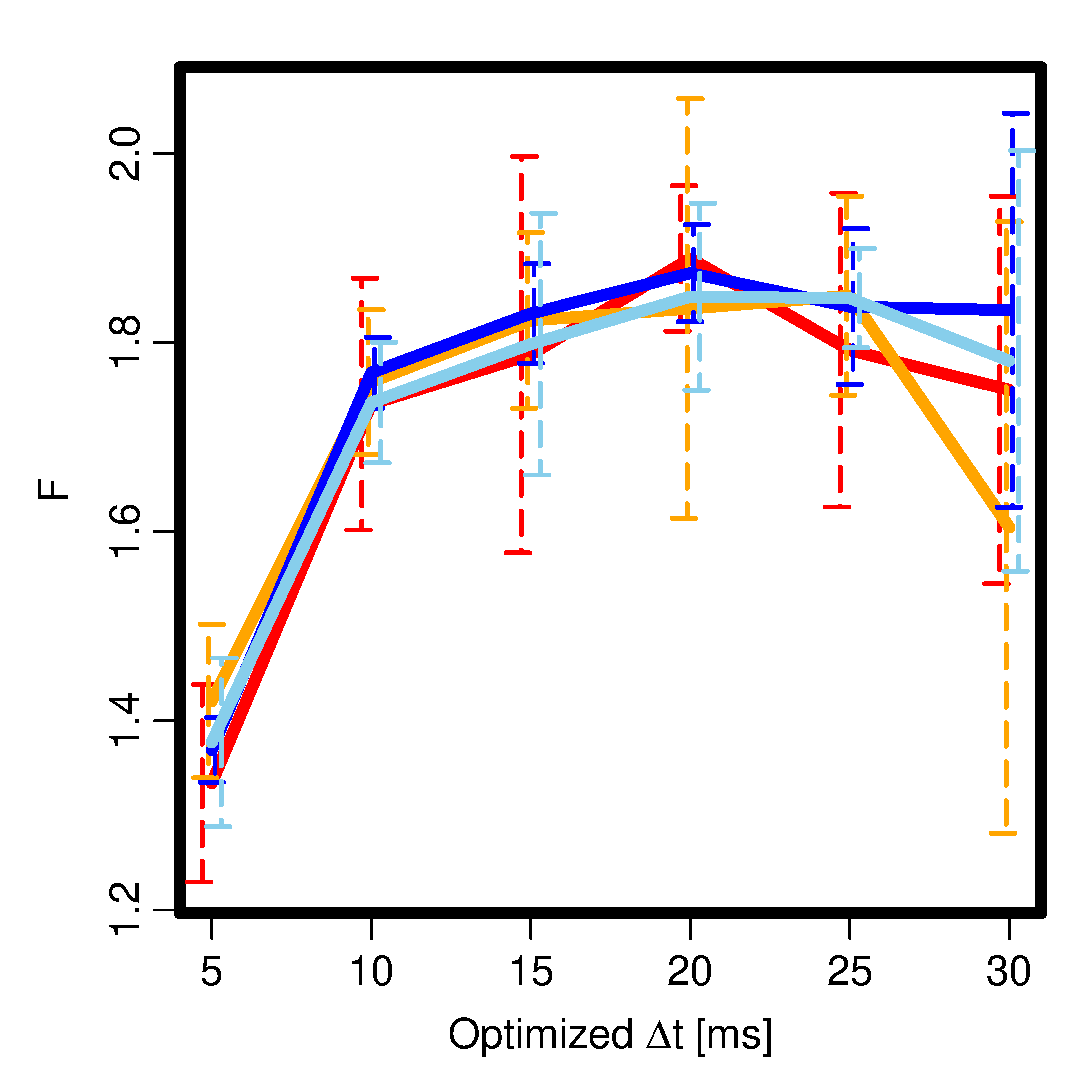
\includegraphics[width=0.8\columnwidth]{./Images_Result/k_ca_test_F.eps}
         \caption{F}
         \label{k_ca_F}
       \end{subfigure}
       \begin{subfigure}{0.5\columnwidth}
         \centering
         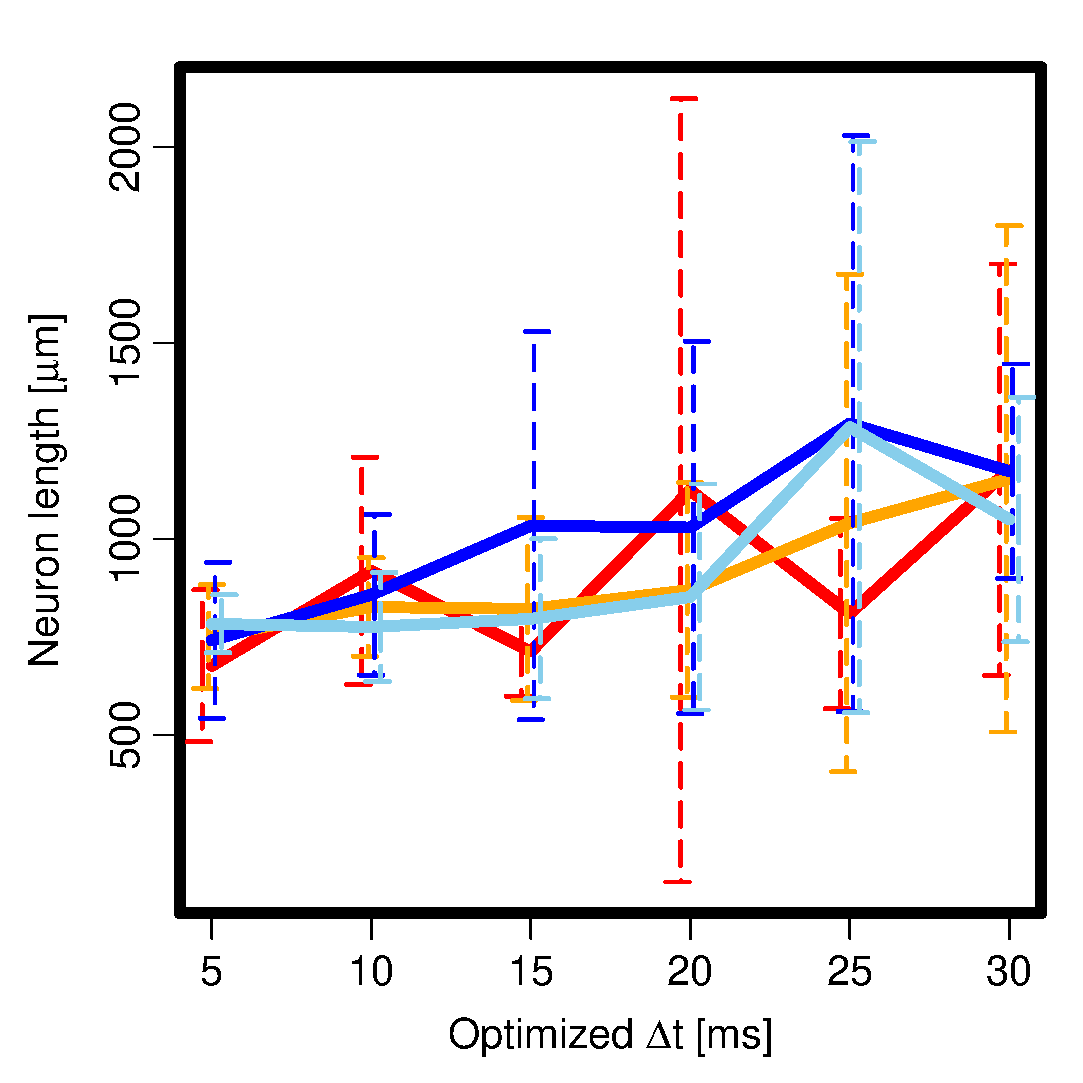
\includegraphics[width=0.8\columnwidth]{./Images_Result/k_ca_test_TREE_length.eps} 
         \caption{$BD9$5(B}
         \label{k_ca_TREE_length}
       \end{subfigure}

       \begin{subfigure}{0.5\columnwidth}
         \centering
         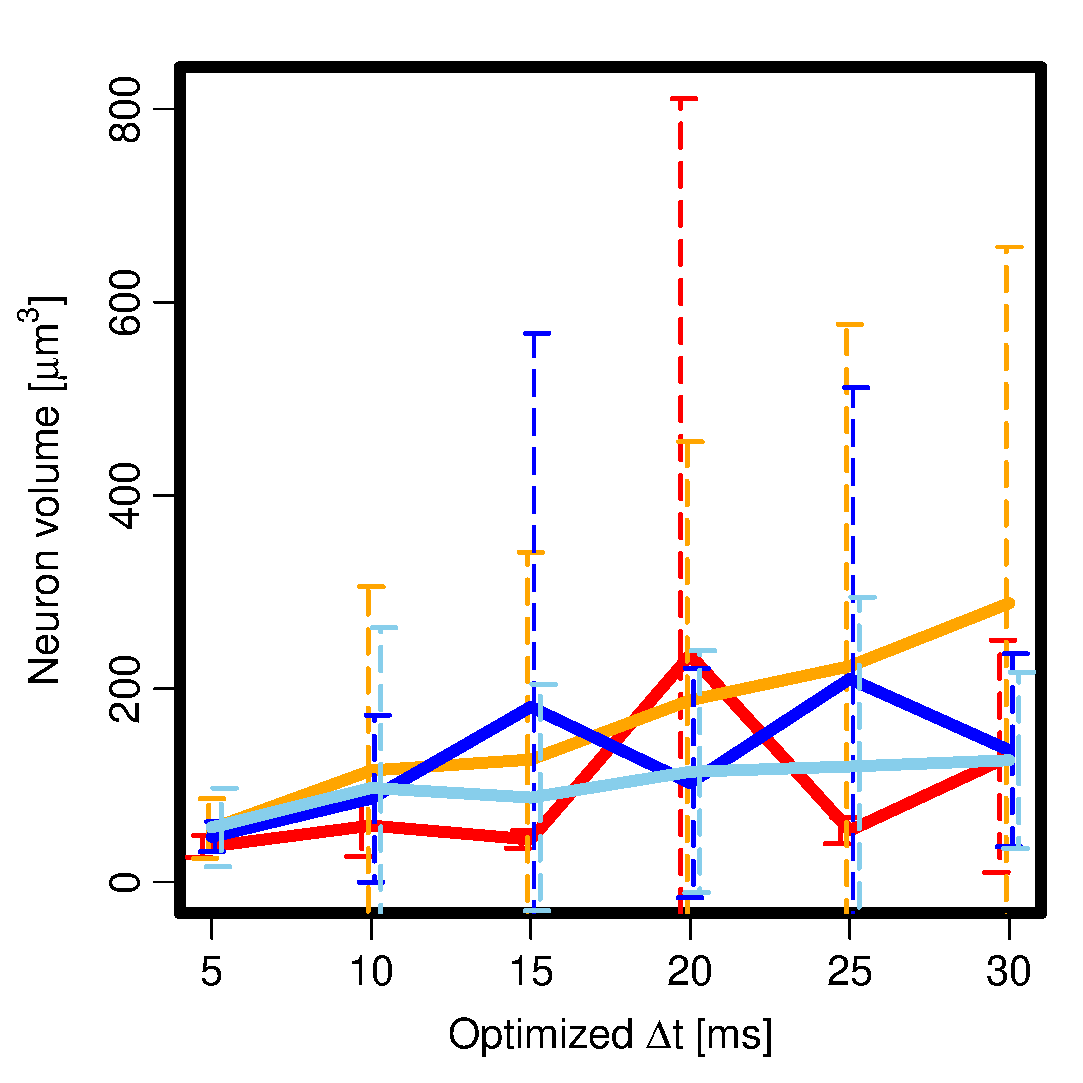
\includegraphics[width=0.8\columnwidth]{./Images_Result/k_ca_test_TREE_volume.eps}
         \caption{$BBN@Q(B}
         \label{k_ca_TREE_volume}
       \end{subfigure}
       \begin{subfigure}{0.5\columnwidth}
         \centering
         \hspace*{-1cm}
         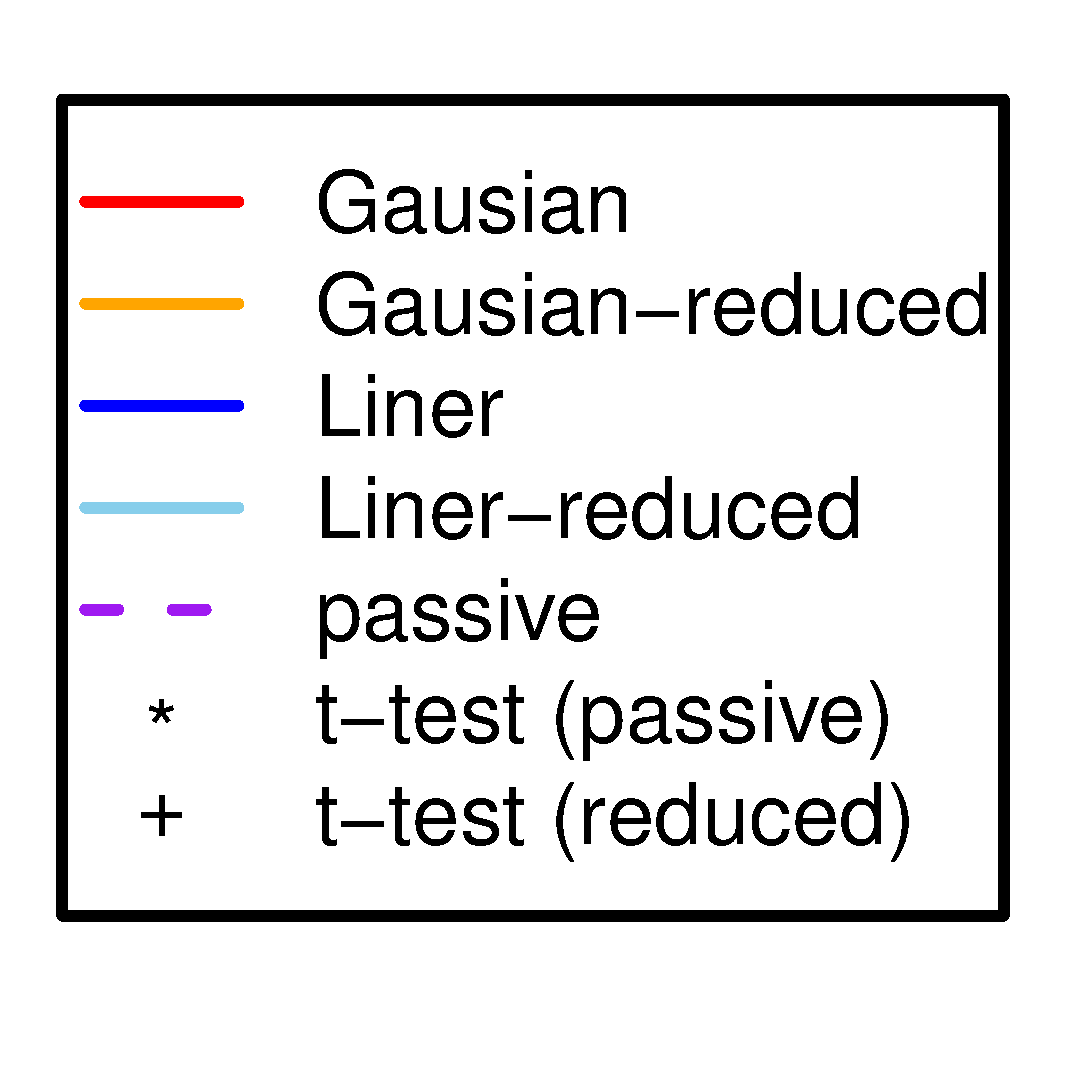
\includegraphics[width=0.5\columnwidth]{./Images_Result/ca_test_legend.eps}
         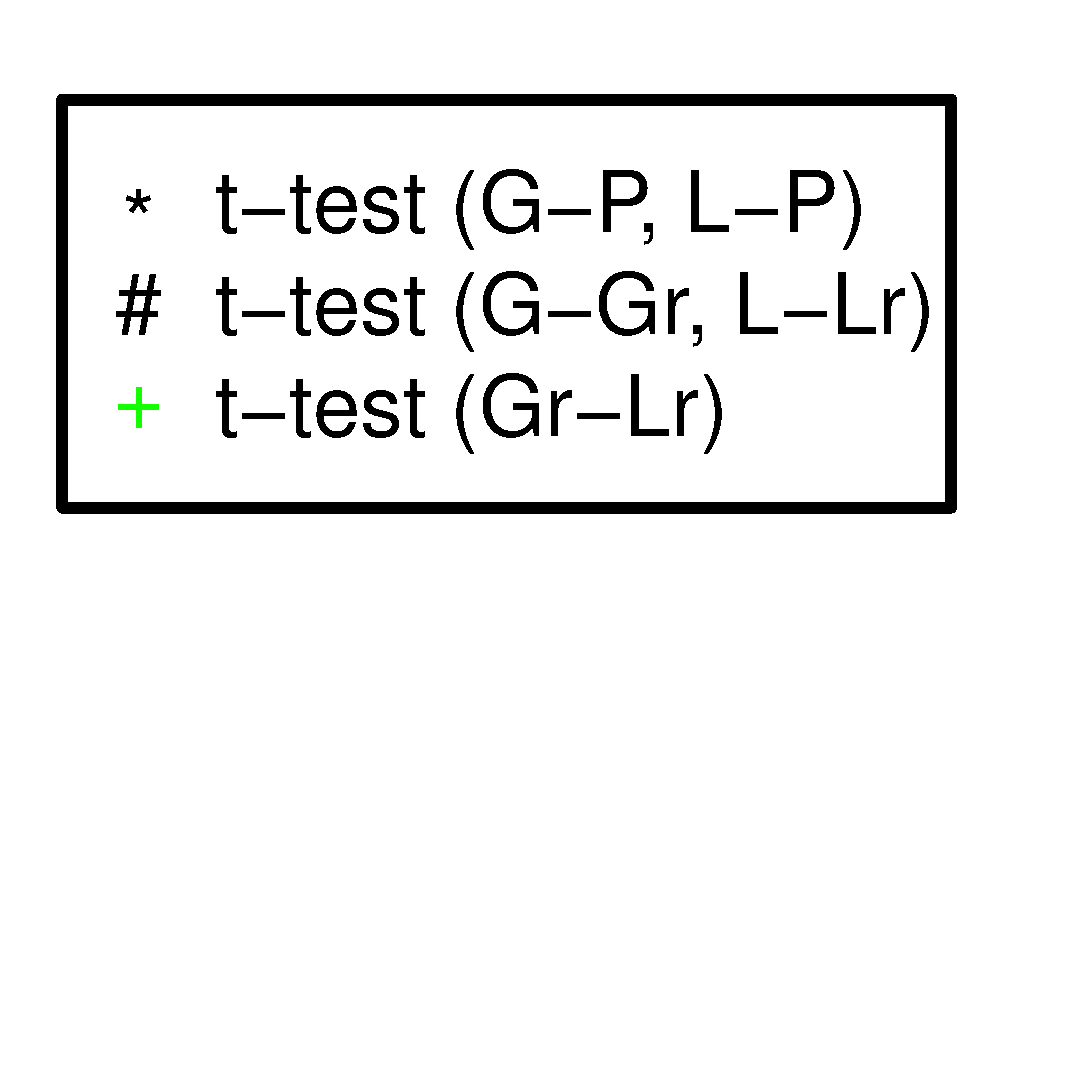
\includegraphics[width=0.5\columnwidth]{./Images_Result/test_legend.eps} 
       \end{subfigure}
              
       \caption{Ka$B%A%c%M%k(B, CaT$B%A%c%M%k$rF3F~$7$?:]$N7k2L(B1} %$B%Z!<%8%l%$%"%&%H$,7hDj$7$F$+$iHyD4@0$9$k(B
       \label{k_ca_result1}
     \end{figure}

     \begin{figure}
       \begin{subfigure}{0.5\columnwidth}
         \centering
         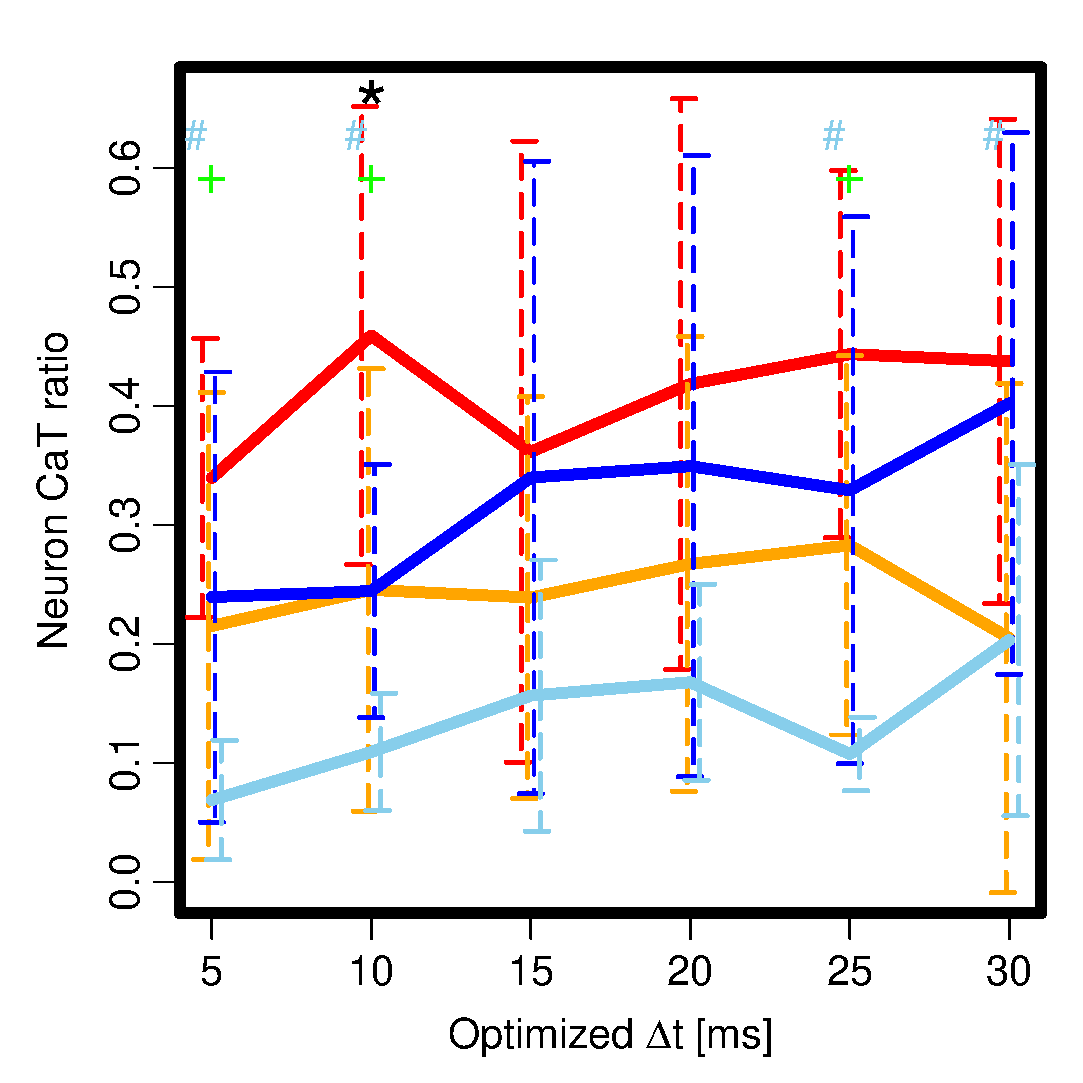
\includegraphics[width=0.8\columnwidth]{./Images_Result/k_ca_test_TREE_Ca_ratio.eps}
         \caption{CaT$B%3%s%@%/%?%s%94^M-N((B}
         \label{ca_TREE_Ca_ratio}
       \end{subfigure}
       \begin{subfigure}{0.5\columnwidth}
         \centering
         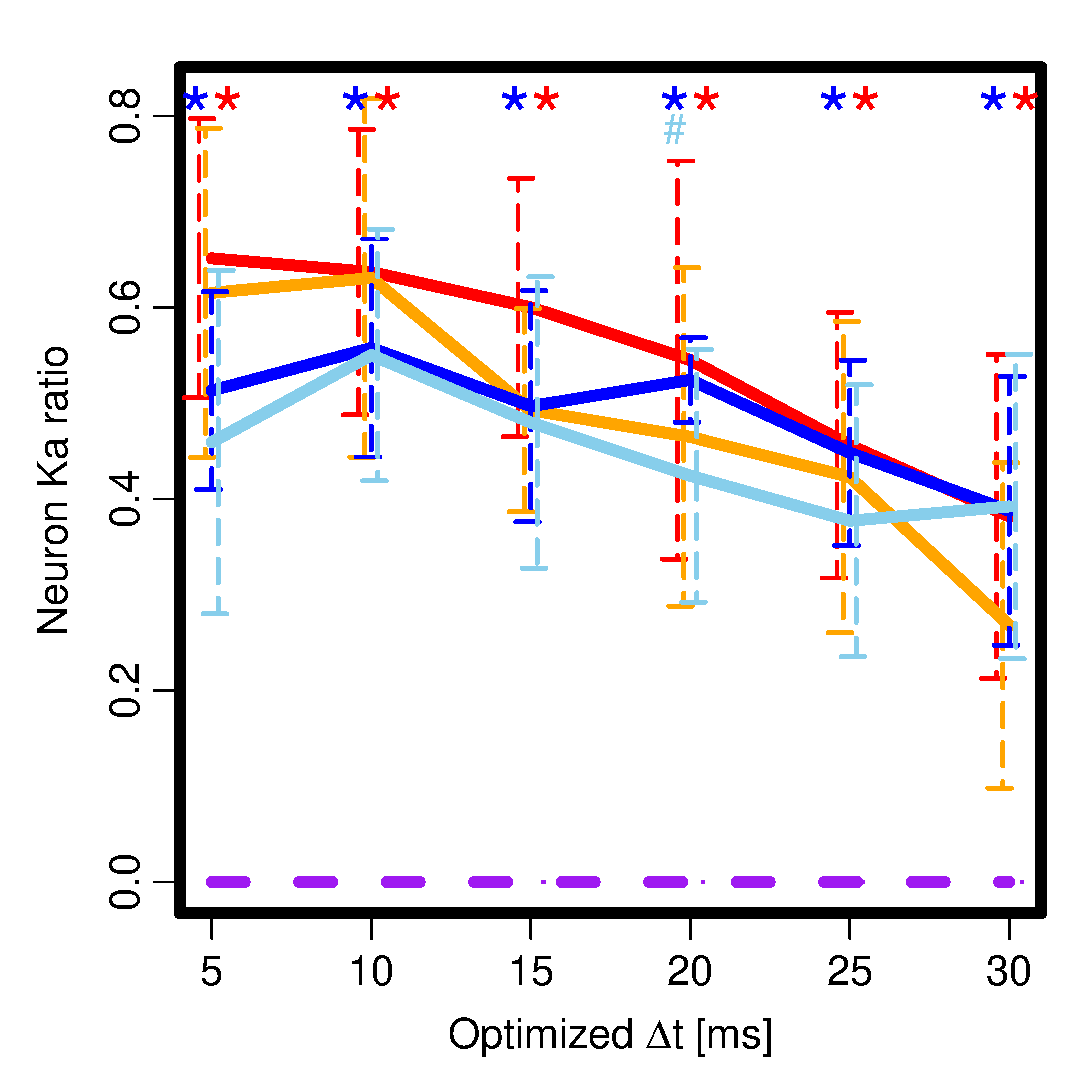
\includegraphics[width=0.8\columnwidth]{./Images_Result/k_ca_test_TREE_K_ratio.eps}
         \caption{Ka$B%3%s%@%/%?%s%94^M-N((B}
         \label{ca_TREE_K_ratio}
       \end{subfigure}
       
       \begin{subfigure}{0.5\columnwidth}
         \centering
         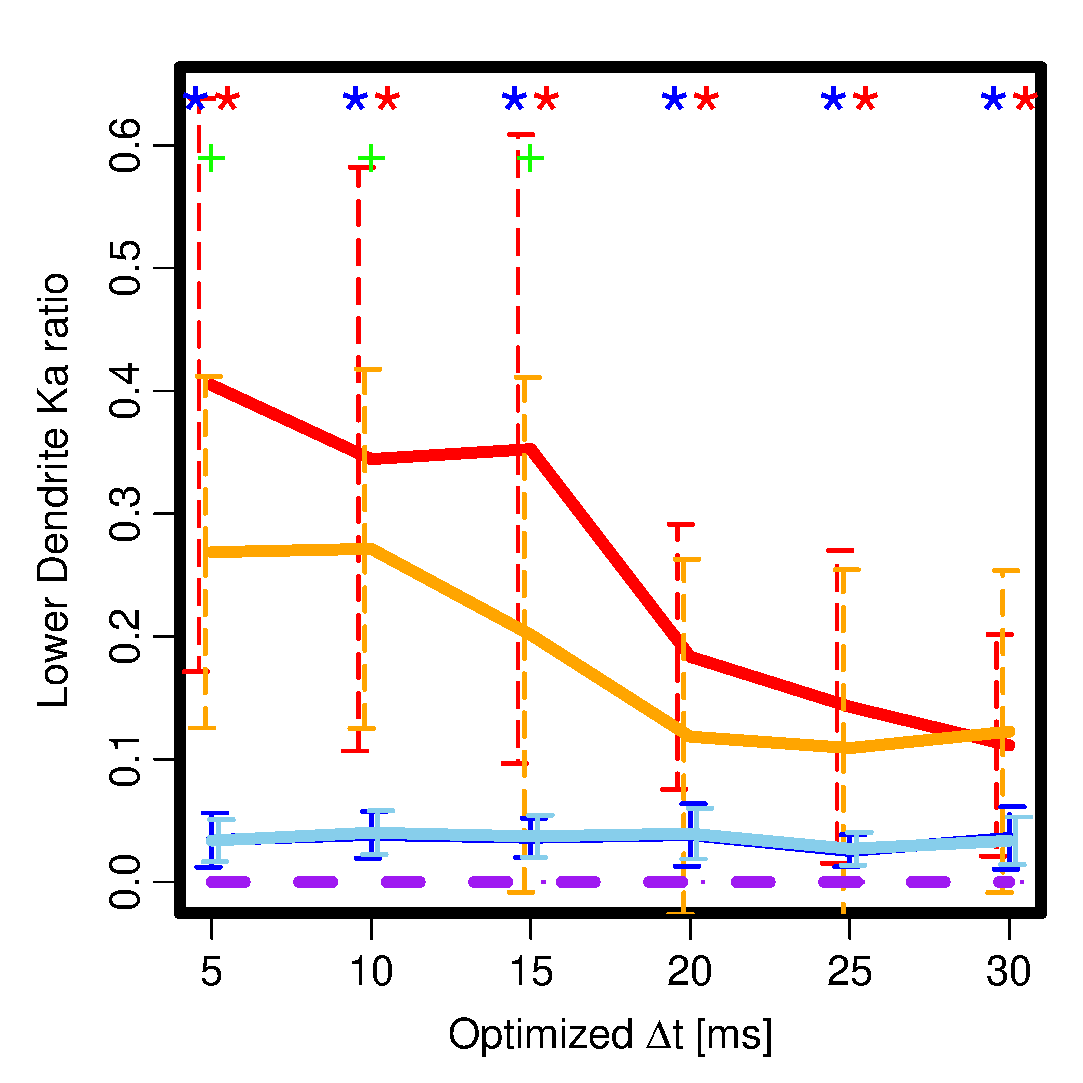
\includegraphics[width=0.8\columnwidth]{./Images_Result/k_ca_test_Lower_K_ratio.eps}
         \caption{Lower Dendrite$B$N(BKa$B%3%s%@%/%?%s%94^M-N((B}
         \label{k_ca_lower_k_ratio}
       \end{subfigure}
       \begin{subfigure}{0.5\columnwidth}
         \centering
         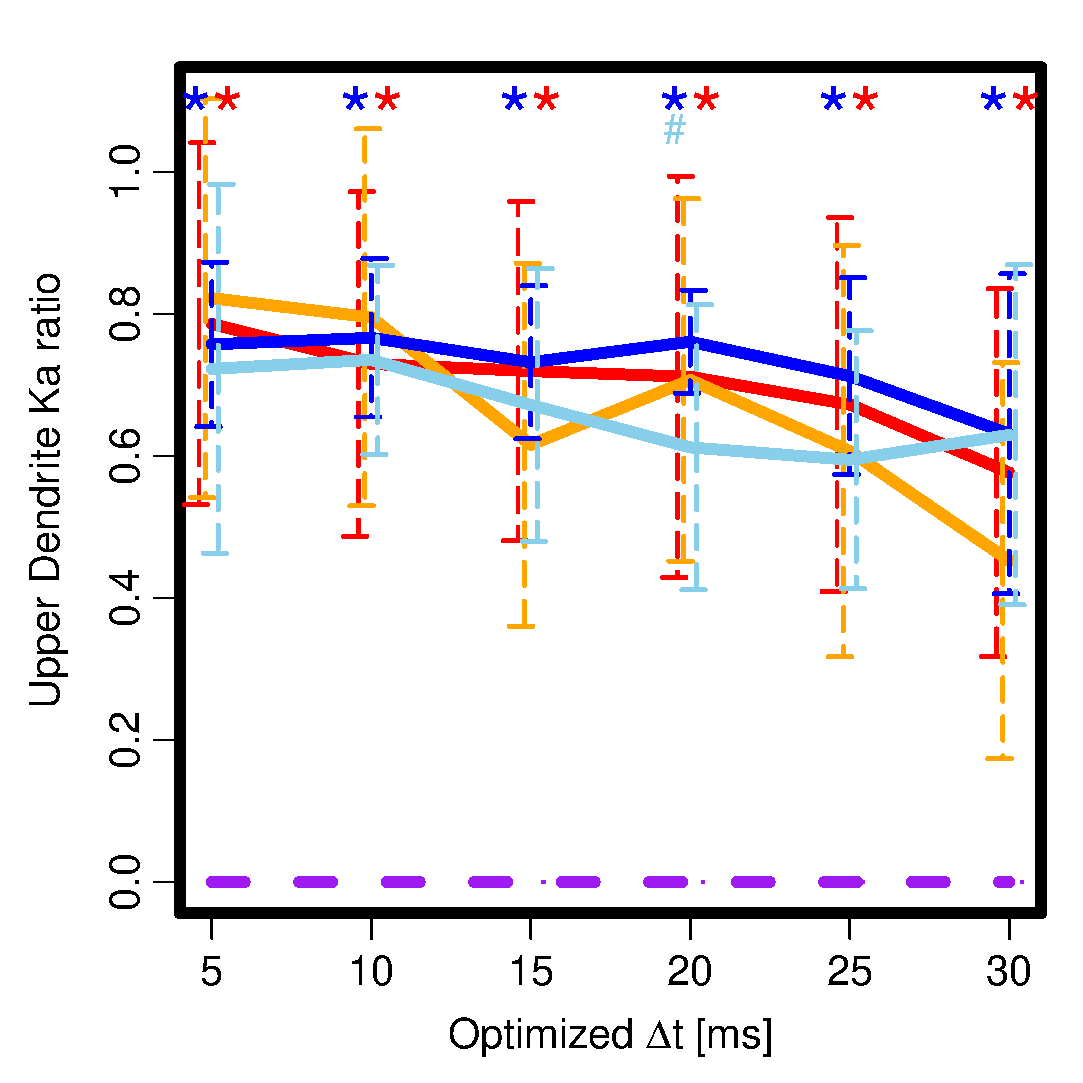
\includegraphics[width=0.8\columnwidth]{./Images_Result/k_ca_test_Upper_K_ratio.eps}
         \caption{Upper Dendrite$B$N(BKa$B%3%s%@%/%?%s%94^M-N((B}
         \label{k_ca_upper_k_ratio}
       \end{subfigure}
       
       \begin{subfigure}{0.5\columnwidth}
         \centering
         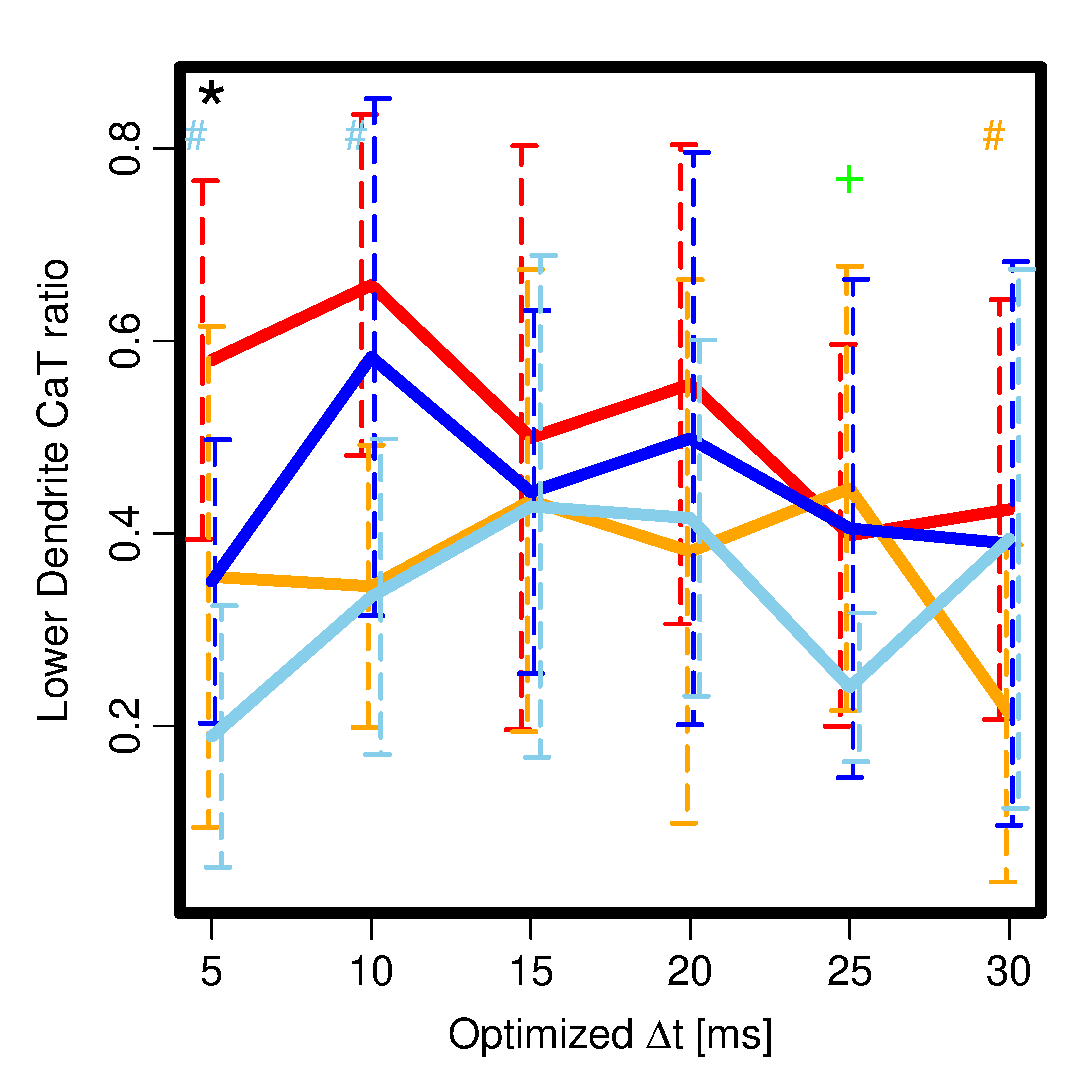
\includegraphics[width=0.8\columnwidth]{./Images_Result/k_ca_test_Lower_Ca_ratio.eps}
         \caption{Lower Dendrite$B$N(BCaT$B%3%s%@%/%?%s%94^M-N((B}
         \label{k_ca_lower_ca_ratio}
       \end{subfigure}
       \begin{subfigure}{0.5\columnwidth}
         \centering
         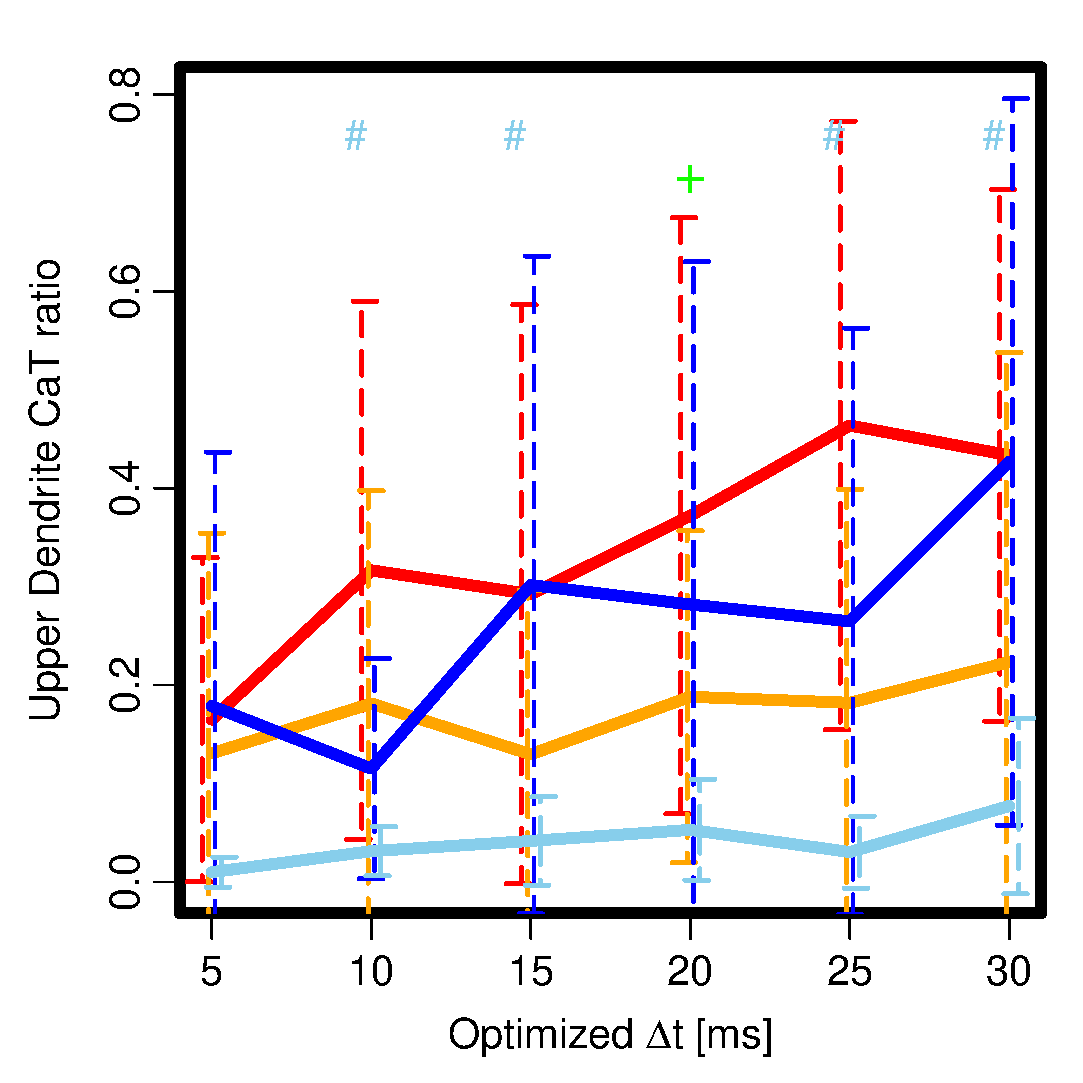
\includegraphics[width=0.8\columnwidth]{./Images_Result/k_ca_test_Upper_Ca_ratio.eps}
         \caption{Upper Dendrite$B$N(BCaT$B%3%s%@%/%?%s%94^M-N((B}
         \label{k_ca_upper_ca_ratio}
       \end{subfigure}

       \caption{Ka$B%A%c%M%k(B, CaT$B%A%c%M%k$rF3F~$7$?:]$N7k2L(B2} %$B%Z!<%8%l%$%"%&%H$,7hDj$7$F$+$iHyD4@0$9$k(B
       \label{k_ca_result2}
     \end{figure}

     %% \begin{figure}[H]
     %%   \begin{subfigure}{0.5\columnwidth}
     %%     \centering
     %%     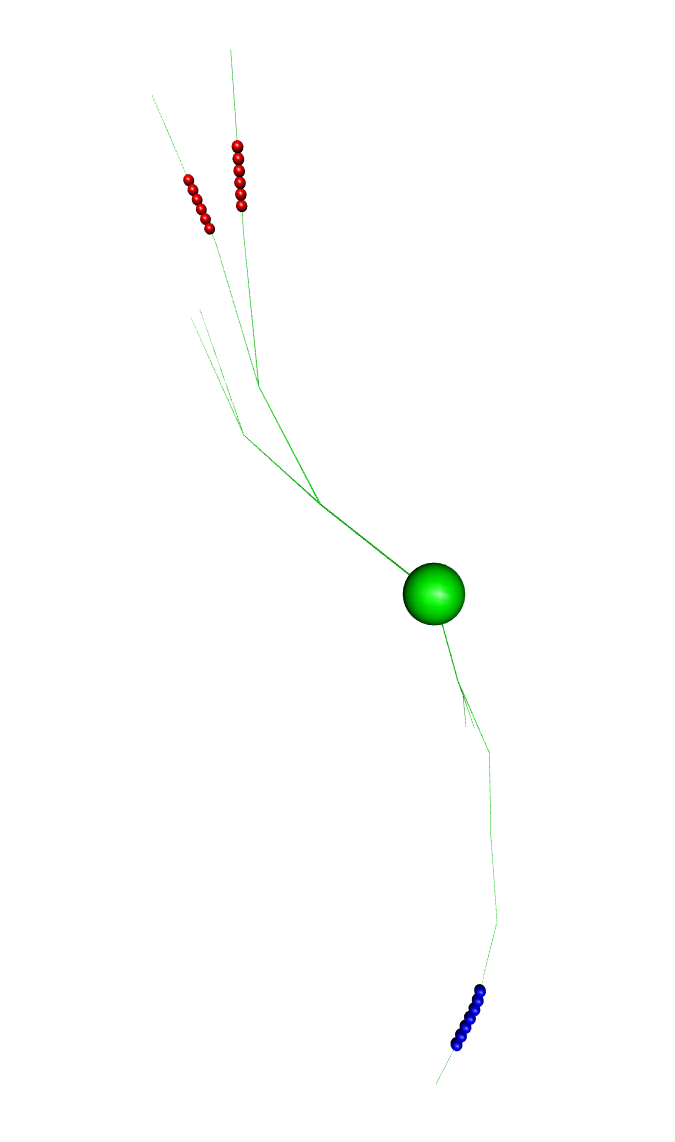
\includegraphics[width=0.8\columnwidth]{./Images_Result/k_ca_liner_TREE_sample_dt20_C5.png}
     %%     \caption{$B@~7AJ,I[(B}
     %%     \label{k_ca_liner_morpho}
     %%   \end{subfigure}
     %%          \begin{subfigure}{0.8\columnwidth}
     %%     \centering
     %%     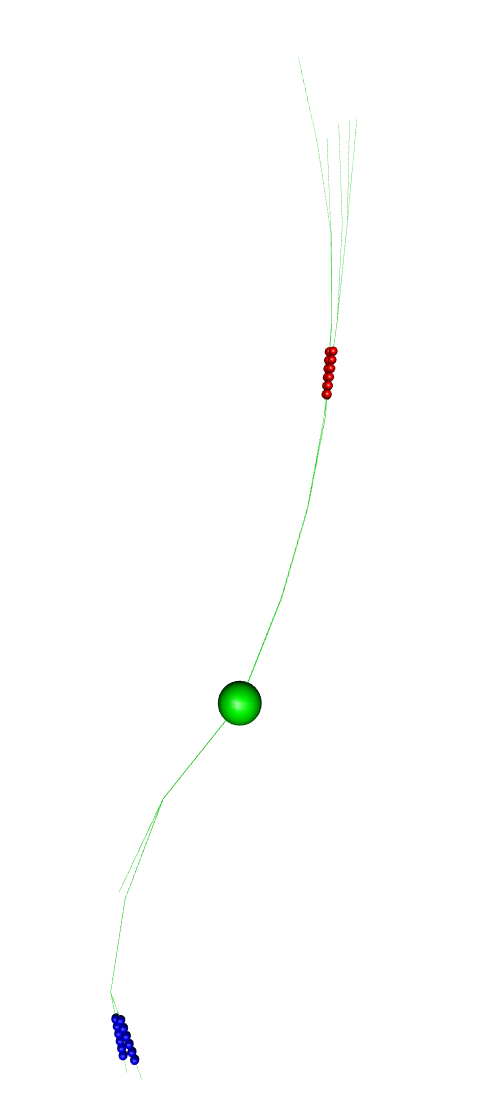
\includegraphics[width=0.8\columnwidth]{./Images_Result/k_ca_gaus_TREE_sample_dt20_C5.png}
     %%     \caption{$B%,%&%9J,I[(B}
     %%     \label{k_ca_gaus_morpho}
     %%   \end{subfigure}

     %%   \caption{Ka$B%A%c%M%k(B, CaT$B%A%c%M%k$rF3F~$7$?:]$N7k2L(B1} %$B%Z!<%8%l%$%"%&%H$,7hDj$7$F$+$iHyD4@0$9$k(B
     %%   \label{k_ca_morpho}
     %% \end{figure}

     \begin{figure}[H]
       \hspace*{-2cm}
       \begin{subfigure}{0.62\columnwidth}
         \centering
         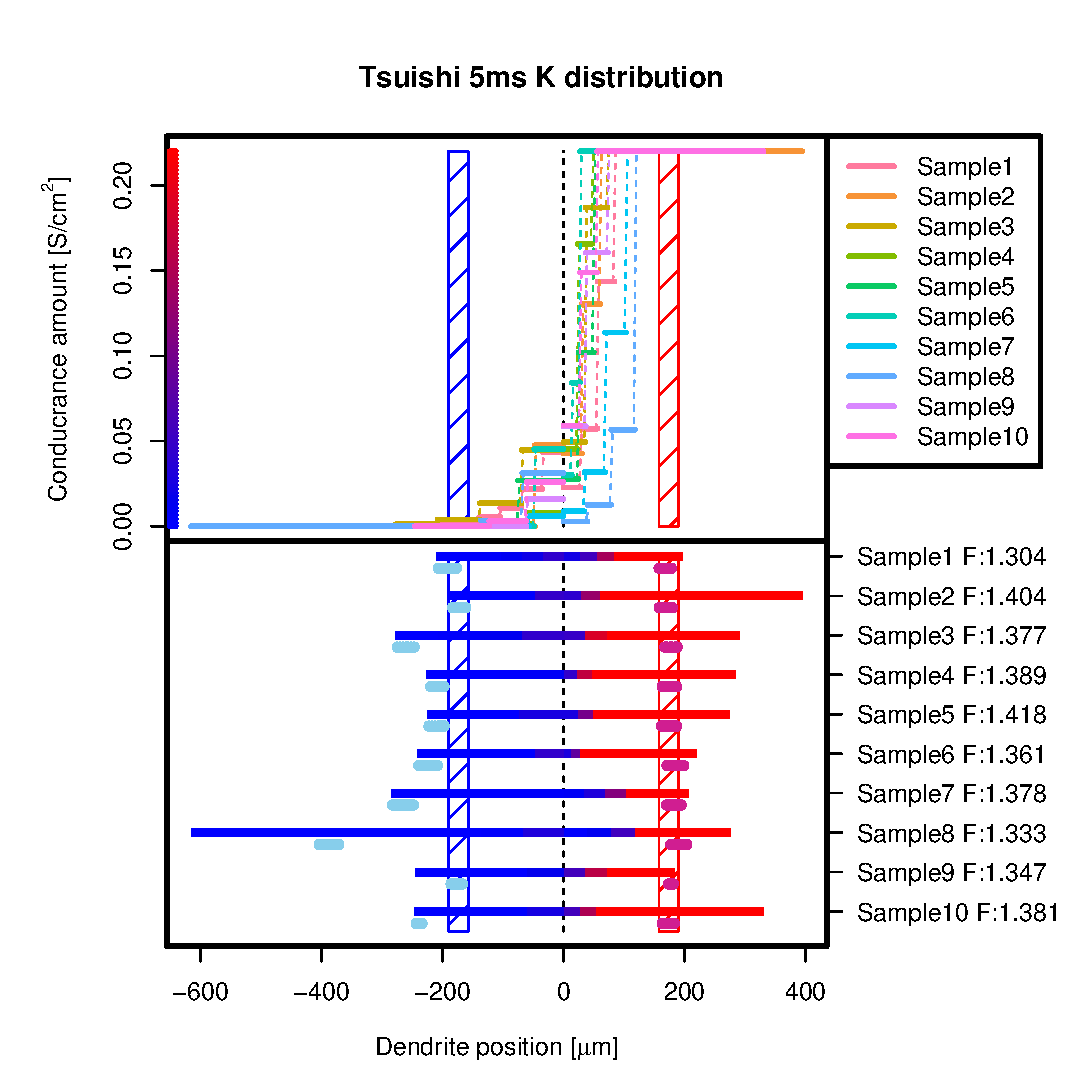
\includegraphics[width=\columnwidth]{./Images_Result/k_ca_Rerative_liner_75_0_K_distribution_dt5.eps}
         \caption{$B@~7AJ,I[(B}
         \label{k_liner_reduced_dist}
       \end{subfigure}
       \begin{subfigure}{0.62\columnwidth}
         \centering
         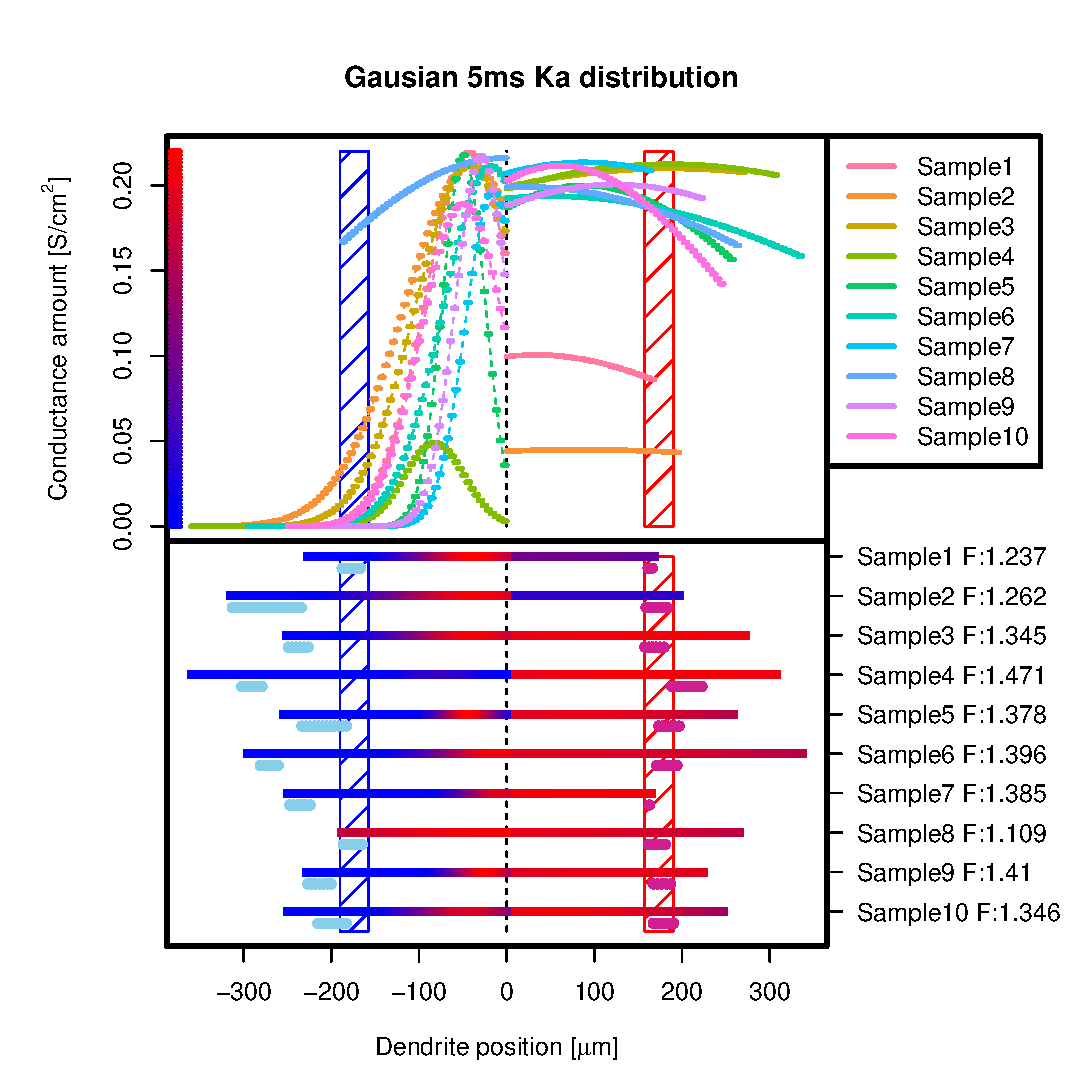
\includegraphics[width=\columnwidth]{./Images_Result/k_ca_Rerative_Gaus_75_0_K_distribution_dt5.eps}
         \caption{$B%,%&%9J,I[(B}
         \label{k_gaus_reduced_dist}
       \end{subfigure}

       \hspace*{-2cm}
       \begin{subfigure}{0.62\columnwidth}
         \centering
         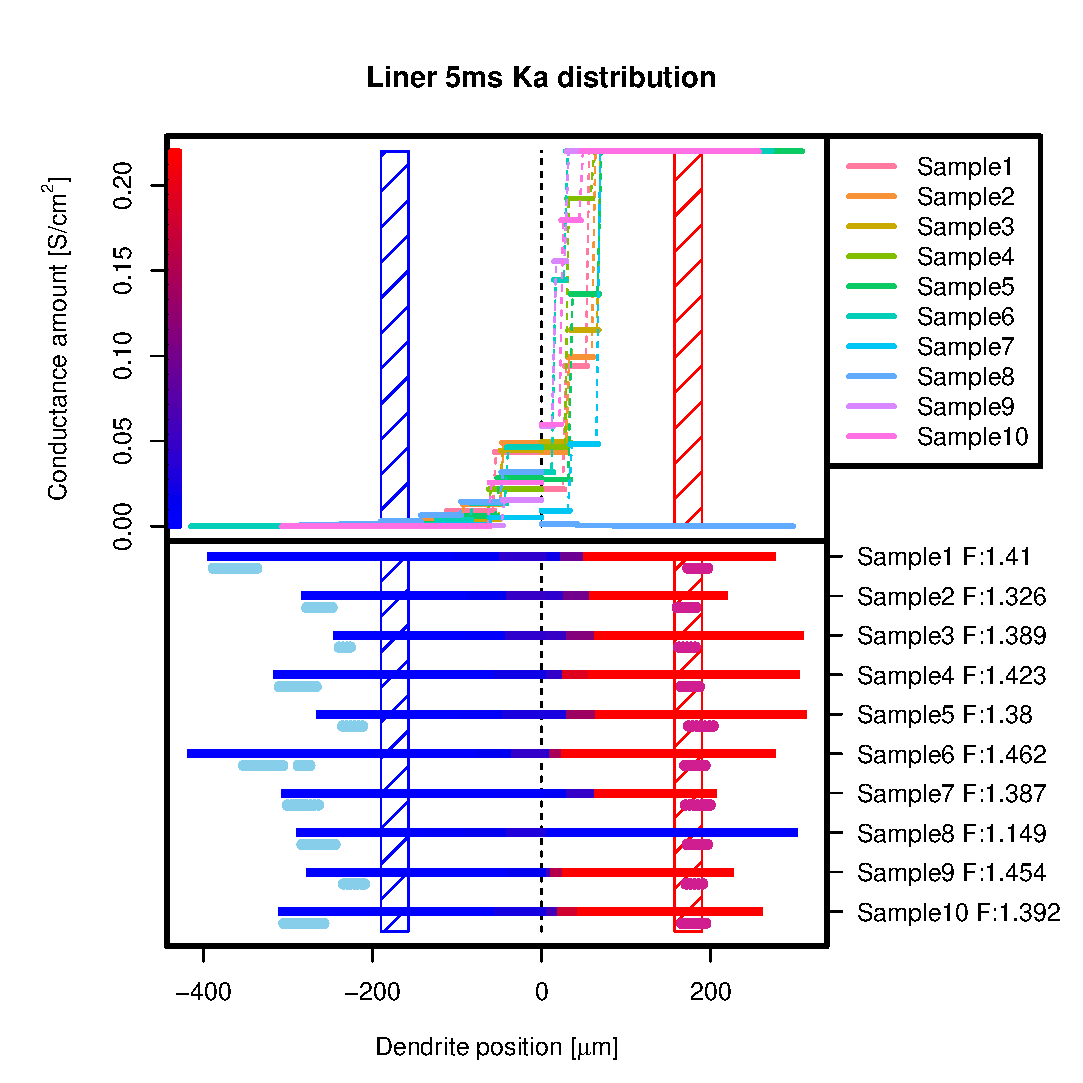
\includegraphics[width=\columnwidth]{./Images_Result/k_ca_Rerative_liner_75_5_K_distribution_dt5.eps} %$B$3$l$NBjL>$,(BTsuishi$B$K$J$C$F$k(B
         \caption{$B@~7AJ,I[(B(reduced)}
         \label{k_liner_reduced_dist}
       \end{subfigure}
       \begin{subfigure}{0.62\columnwidth}
         \centering
         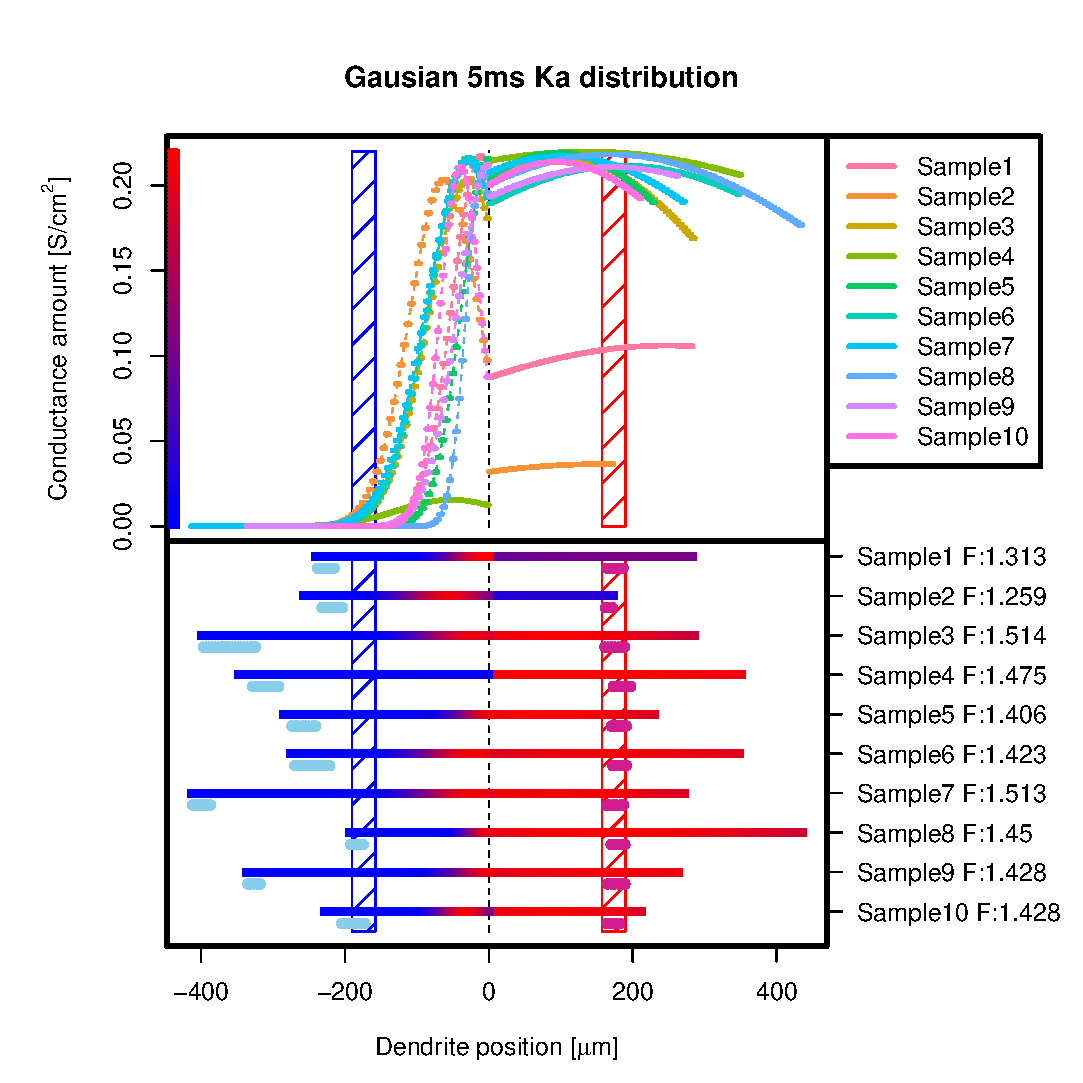
\includegraphics[width=\columnwidth]{./Images_Result/k_ca_Rerative_Gaus_75_5_K_distribution_dt5.eps}
         \caption{$B%,%&%9J,I[(B(reduced)}
         \label{k_gaus_reduced_dist}
       \end{subfigure}
       
       \begin{subfigure}{\columnwidth}
         \centering
         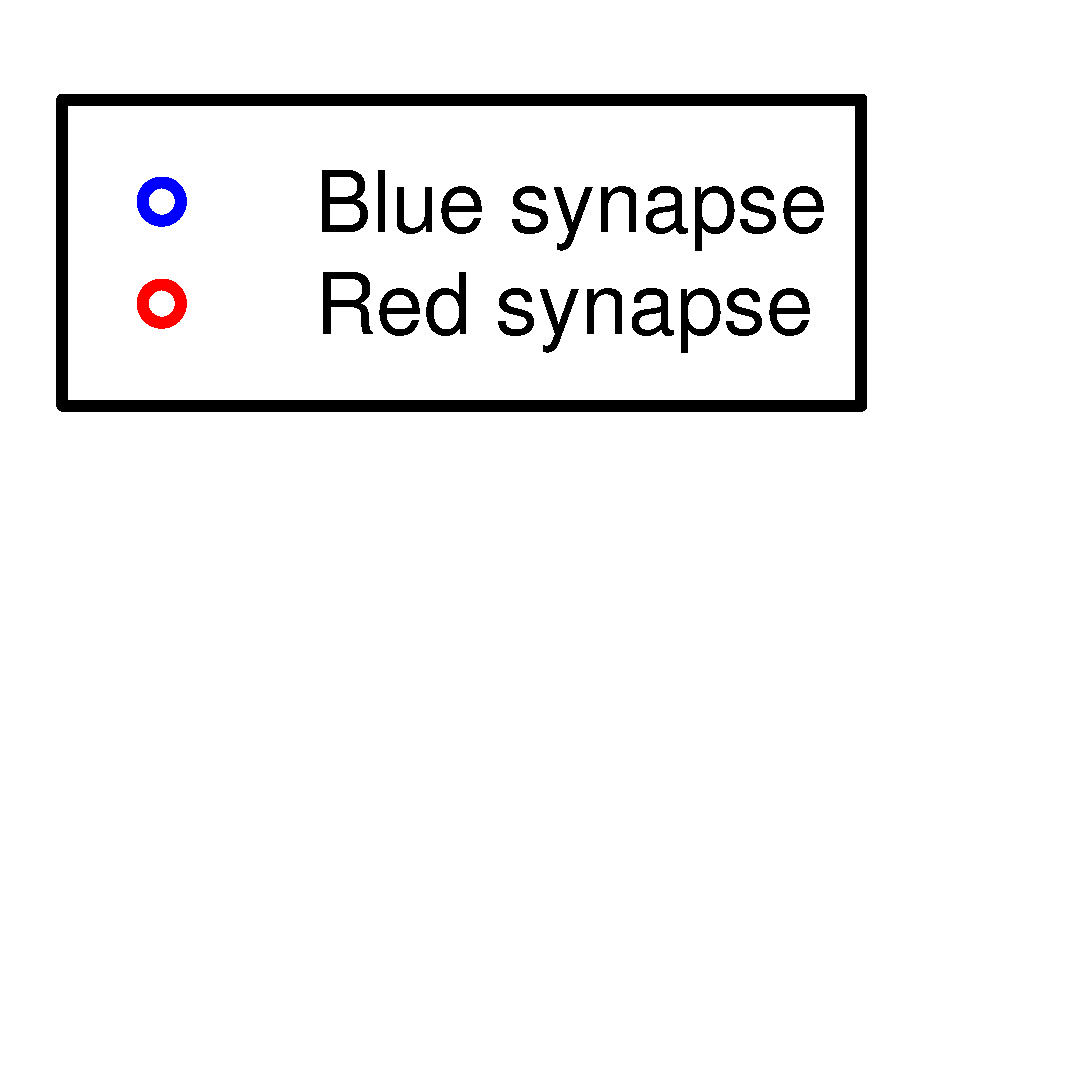
\includegraphics[width=0.35\columnwidth]{./Images_Result/Synapse_legend.eps} 
       \end{subfigure}
       
       \vspace{-3cm}
       \caption{${\Delta}t = 5$[ms], $B$G$N(BKa$B%3%s%@%/%?%s%9J,I[(B}
       \label{k_Ka_dist}
     \end{figure}

     \begin{figure}[H]
       \hspace*{-2cm}
       \begin{subfigure}{0.62\columnwidth}
         \centering
         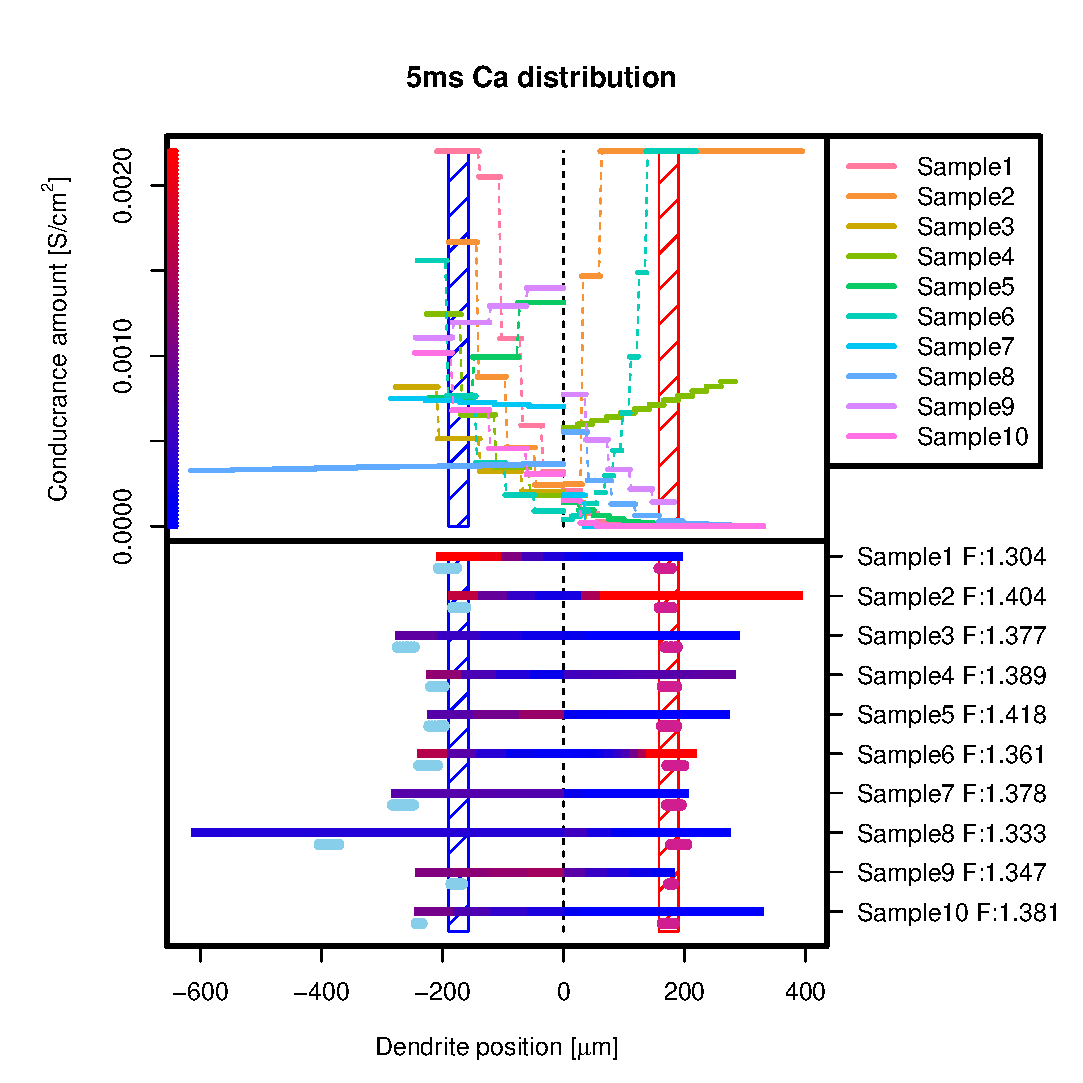
\includegraphics[width=\columnwidth]{./Images_Result/k_ca_Rerative_liner_75_0_Ca_distribution_dt5.eps}
         \caption{$B@~7AJ,I[(B}
         \label{k_liner_reduced_dist}
       \end{subfigure}
       \begin{subfigure}{0.62\columnwidth}
         \centering
         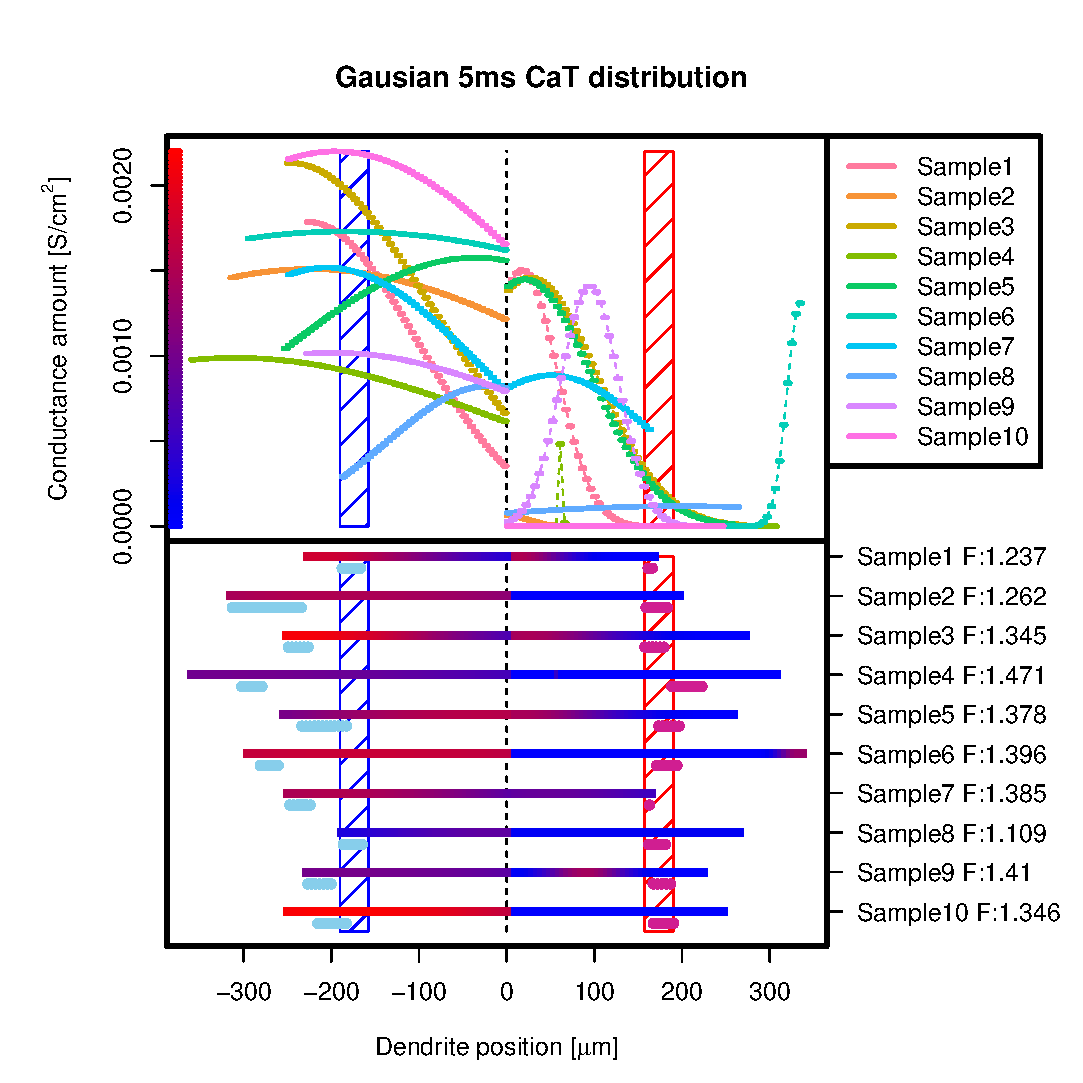
\includegraphics[width=\columnwidth]{./Images_Result/k_ca_Rerative_Gaus_75_0_Ca_distribution_dt5.eps}
         \caption{$B%,%&%9J,I[(B}
         \label{k_gaus_reduced_dist}
       \end{subfigure}

       \hspace*{-2cm}
       \begin{subfigure}{0.62\columnwidth}
         \centering
         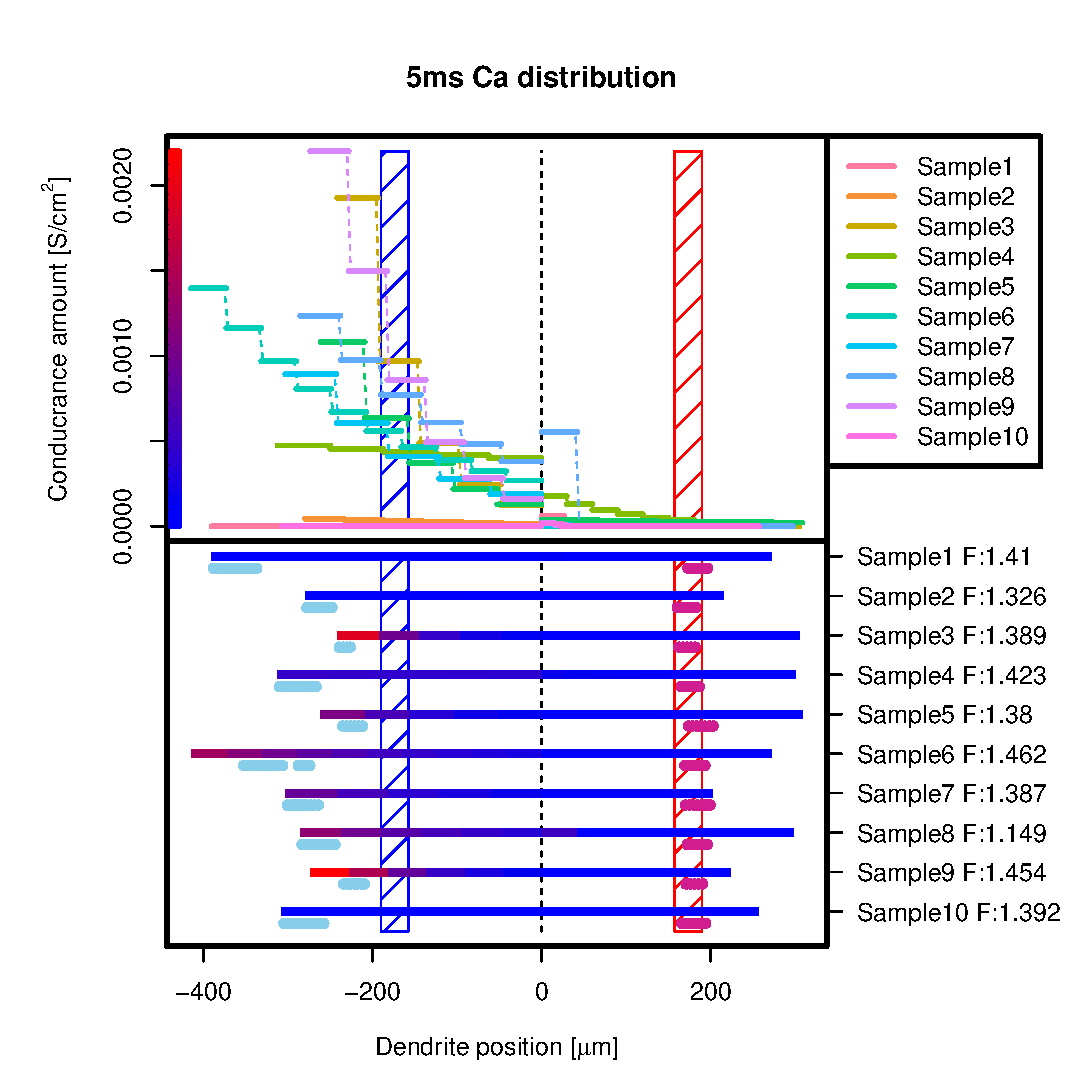
\includegraphics[width=\columnwidth]{./Images_Result/k_ca_Rerative_liner_75_5_Ca_distribution_dt5.eps} %$B$3$l$NBjL>$,(BTsuishi$B$K$J$C$F$k(B
         \caption{$B@~7AJ,I[(B(reduced)}
         \label{k_liner_reduced_dist}
       \end{subfigure}
       \begin{subfigure}{0.62\columnwidth}
         \centering
         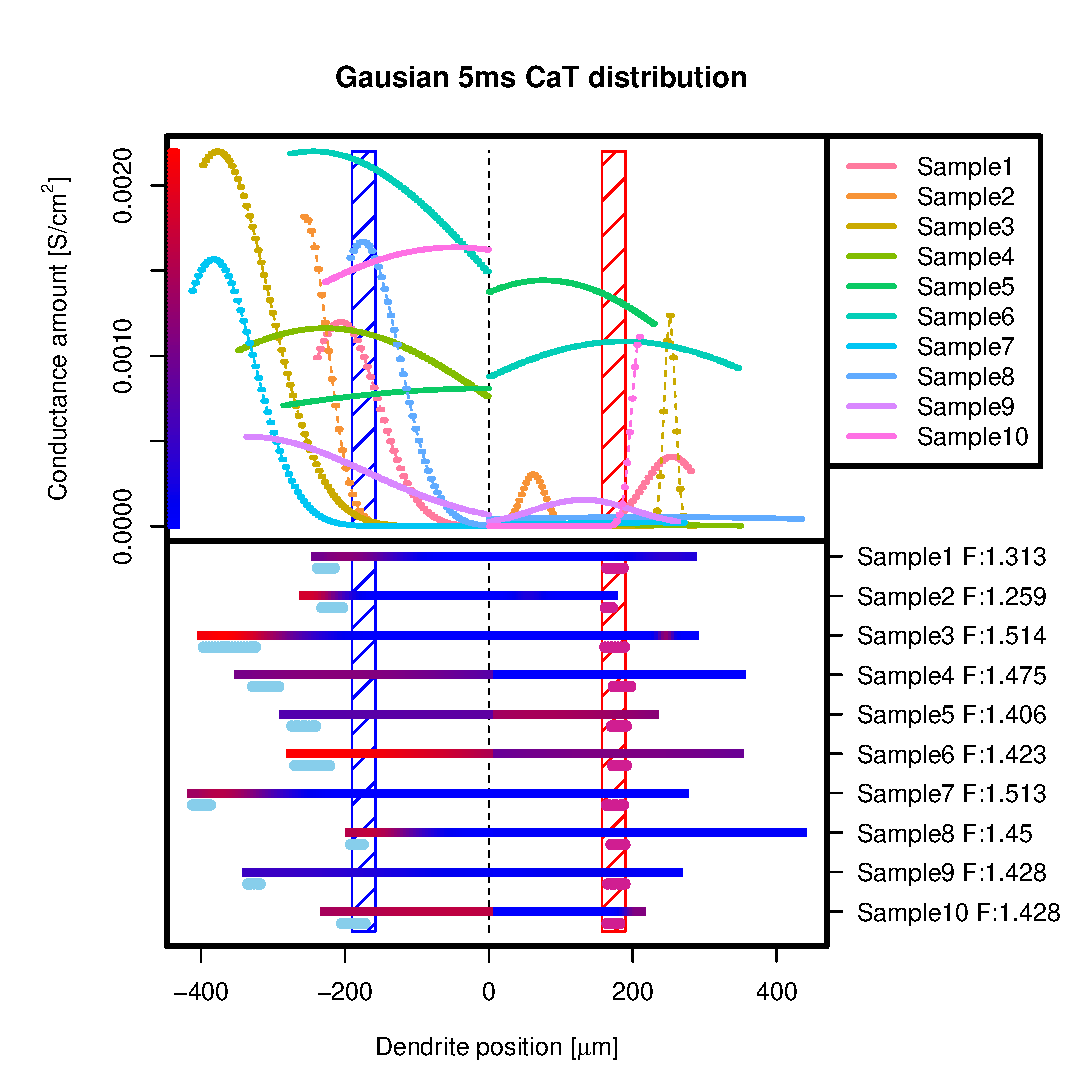
\includegraphics[width=\columnwidth]{./Images_Result/k_ca_Rerative_Gaus_75_5_Ca_distribution_dt5.eps}
         \caption{$B%,%&%9J,I[(B(reduced)}
         \label{k_gaus_reduced_dist}
       \end{subfigure}
       
       \begin{subfigure}{\columnwidth}
         \centering
         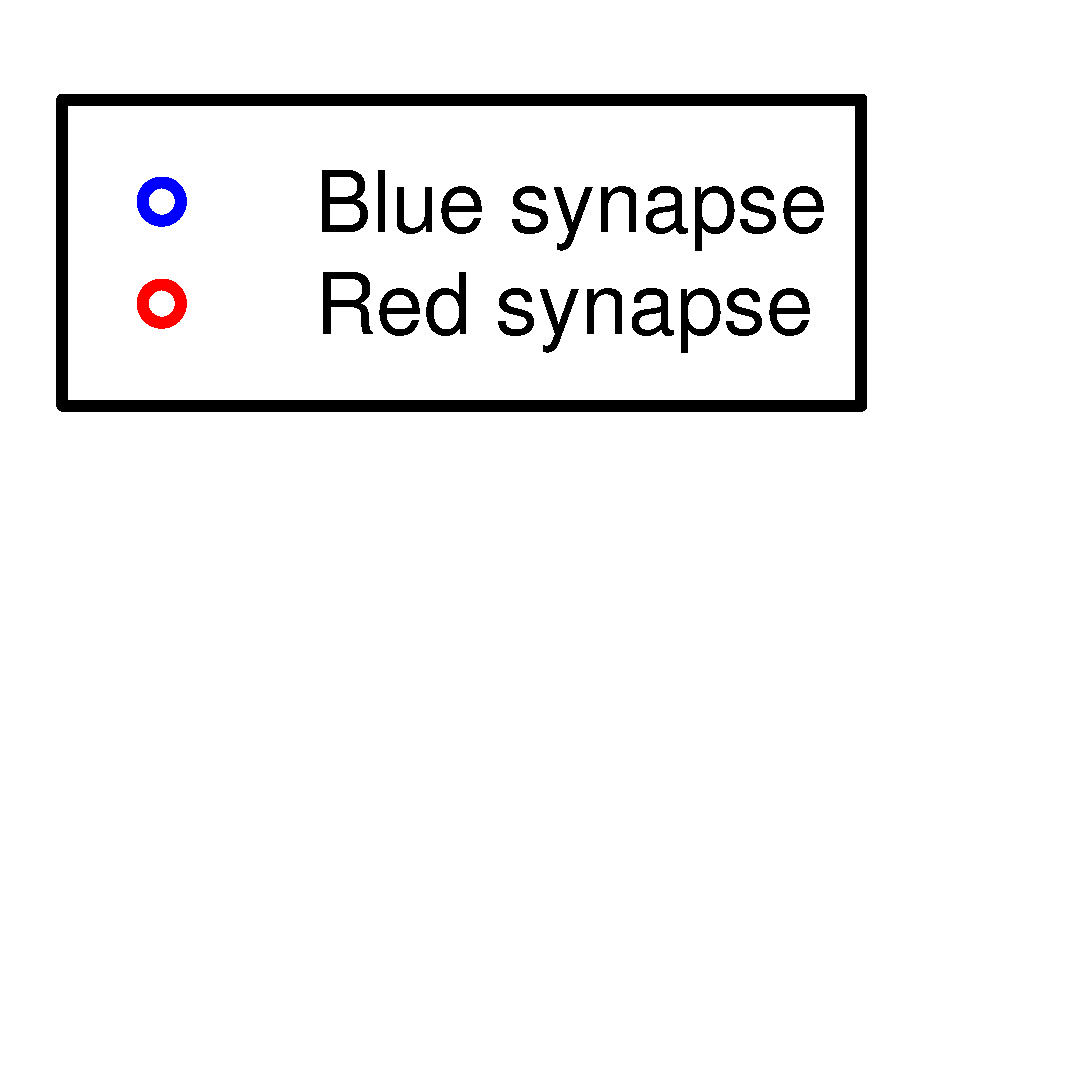
\includegraphics[width=0.35\columnwidth]{./Images_Result/Synapse_legend.eps} 
       \end{subfigure}
       
       \vspace{-3cm}
       \caption{${\Delta}t = 5$[ms], $B$G$N(BCaT$B%3%s%@%/%?%s%9J,I[(B}
       \label{k_CaT_dist}
     \end{figure}

     %------------------------------------------------------------

     \begin{figure}[H]
       \hspace*{-2cm}
       \begin{subfigure}{0.62\columnwidth}
         \centering
         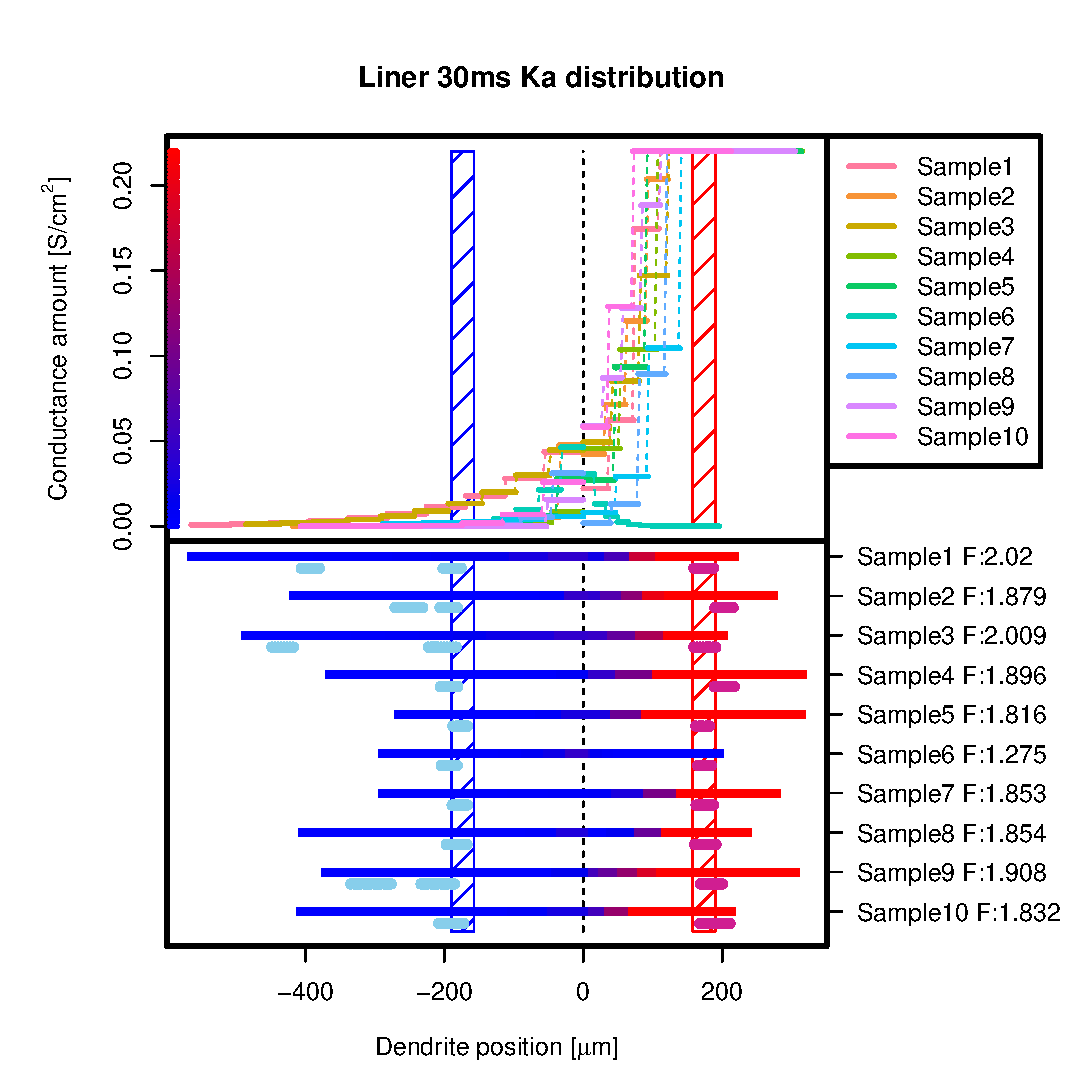
\includegraphics[width=\columnwidth]{./Images_Result/k_ca_Rerative_liner_75_0_K_distribution_dt30.eps}
         \caption{$B@~7AJ,I[(B}
         \label{k_liner_reduced_dist}
       \end{subfigure}
       \begin{subfigure}{0.62\columnwidth}
         \centering
         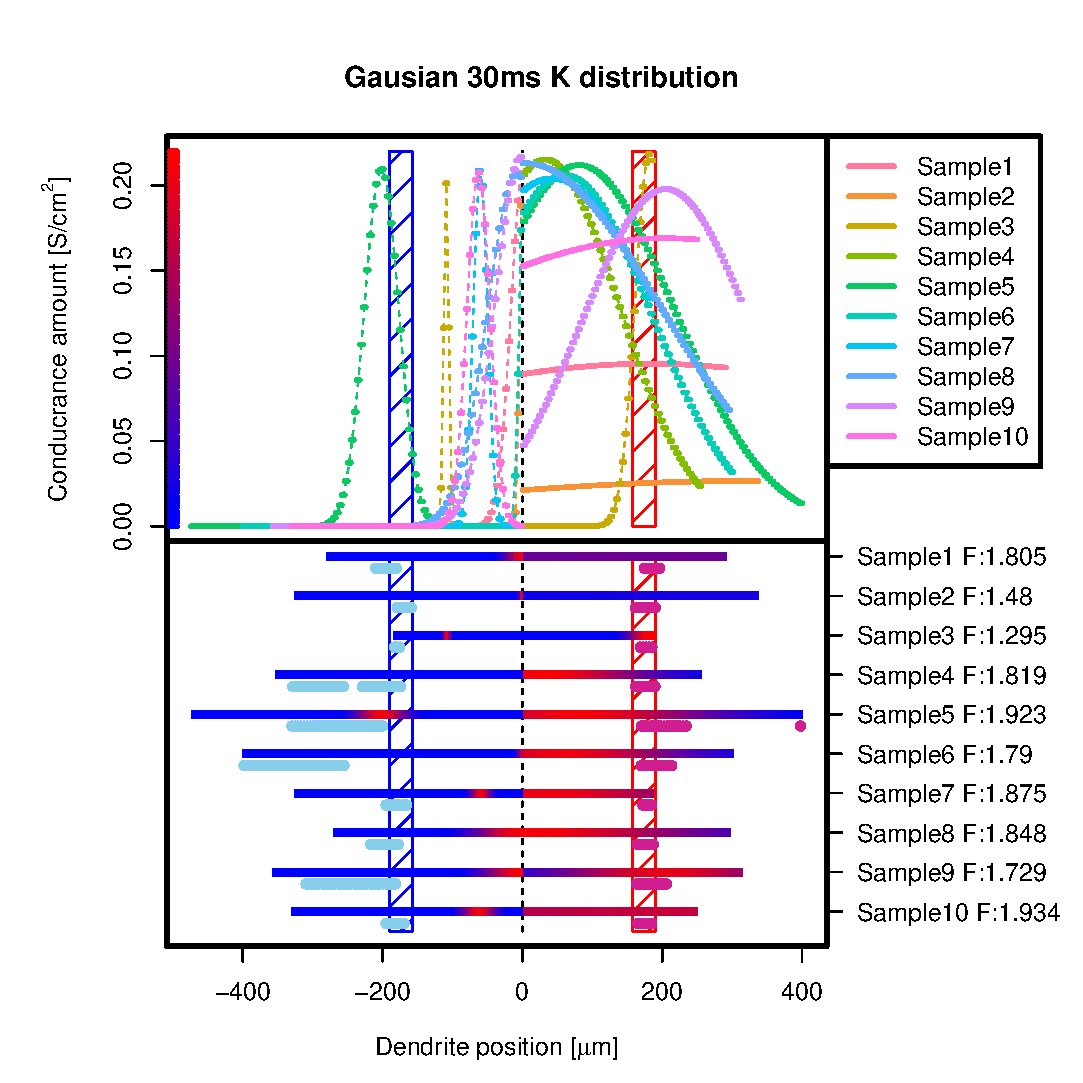
\includegraphics[width=\columnwidth]{./Images_Result/k_ca_Rerative_Gaus_75_0_K_distribution_dt30.eps}
         \caption{$B%,%&%9J,I[(B}
         \label{k_gaus_reduced_dist}
       \end{subfigure}

       \hspace*{-2cm}
       \begin{subfigure}{0.62\columnwidth}
         \centering
         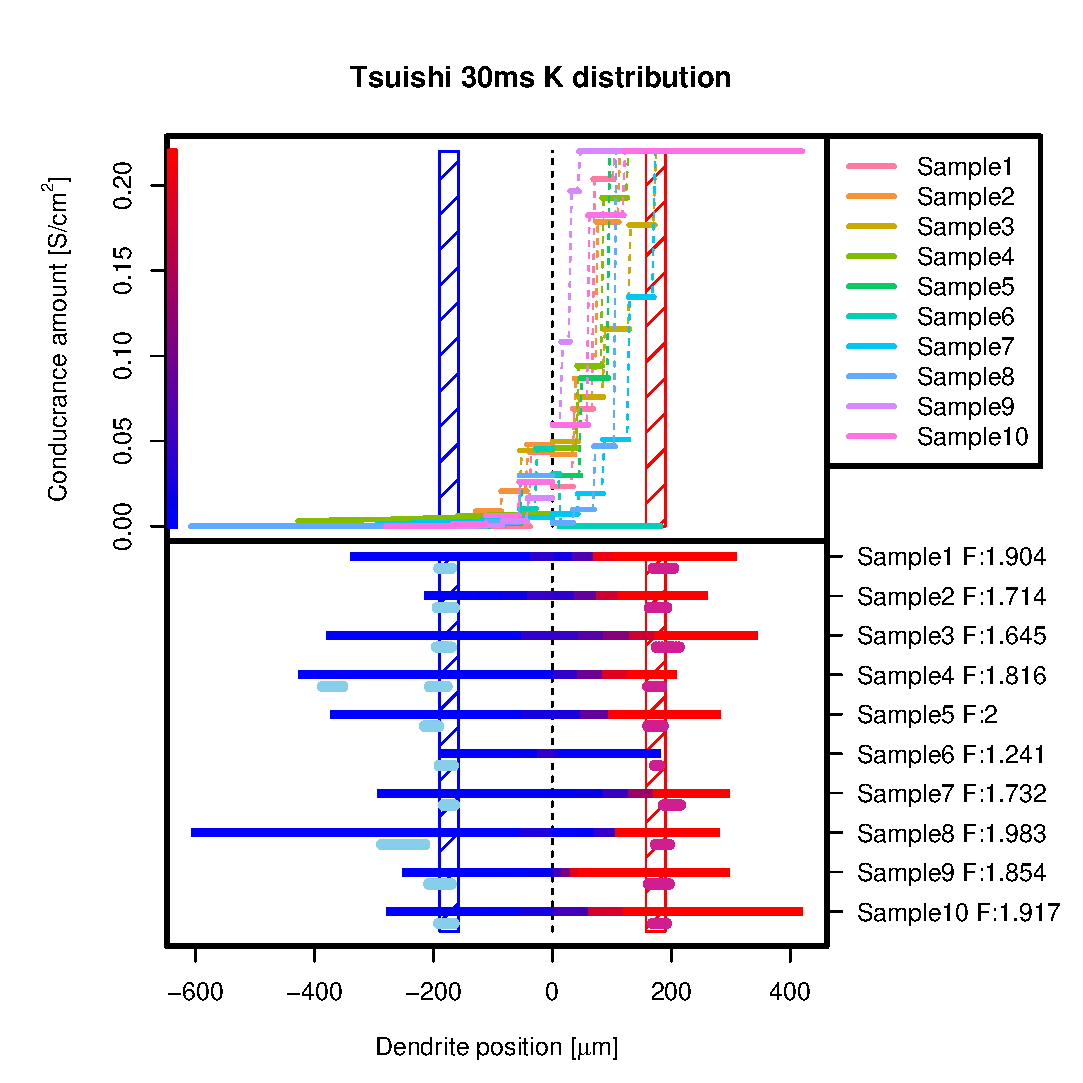
\includegraphics[width=\columnwidth]{./Images_Result/k_ca_Rerative_liner_75_5_K_distribution_dt30.eps} %$B$3$l$NBjL>$,(BTsuishi$B$K$J$C$F$k(B
         \caption{$B@~7AJ,I[(B(reduced)}
         \label{k_liner_reduced_dist}
       \end{subfigure}
       \begin{subfigure}{0.62\columnwidth}
         \centering
         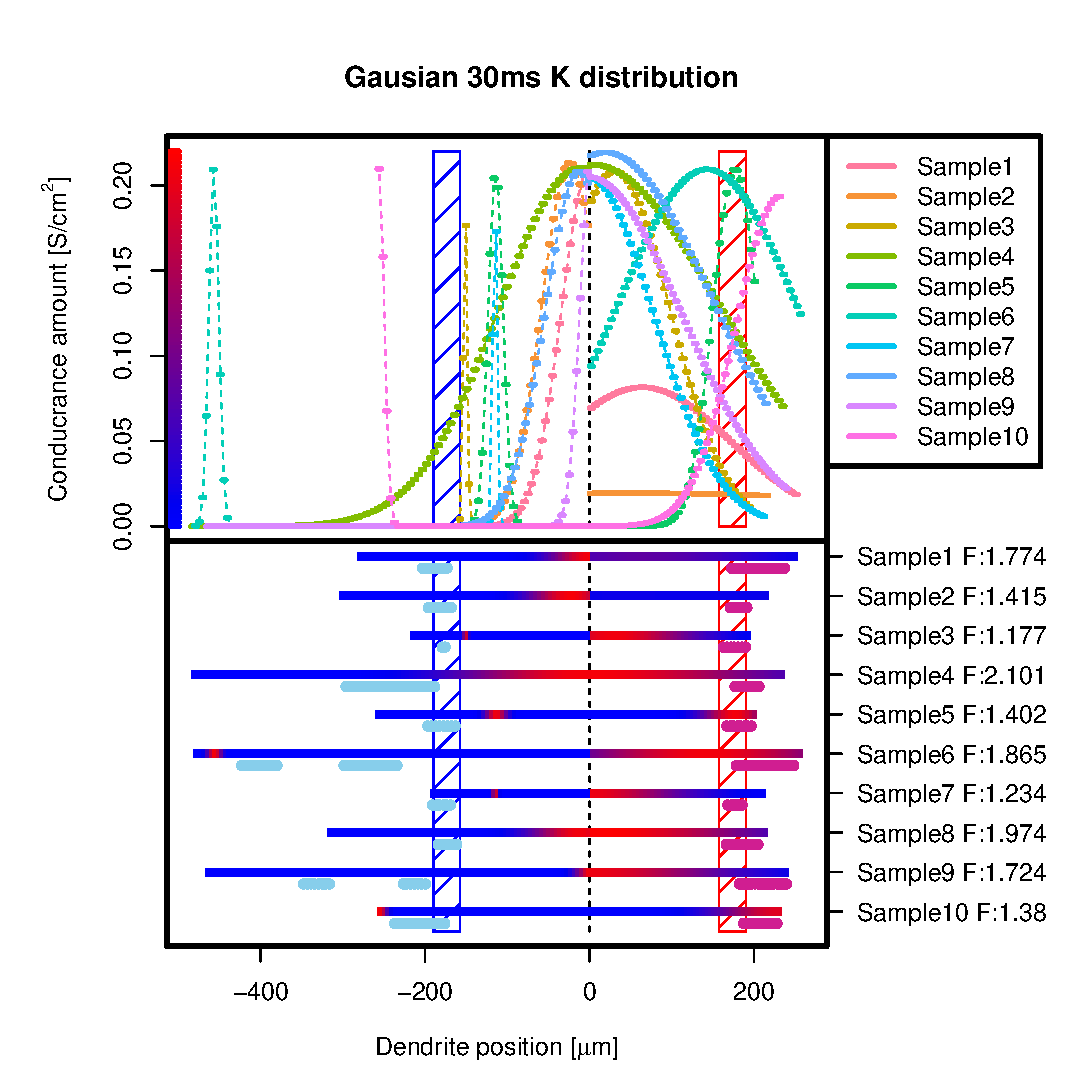
\includegraphics[width=\columnwidth]{./Images_Result/k_ca_Rerative_Gaus_75_5_K_distribution_dt30.eps}
         \caption{$B%,%&%9J,I[(B(reduced)}
         \label{k_gaus_reduced_dist}
       \end{subfigure}
       
       \begin{subfigure}{\columnwidth}
         \centering
         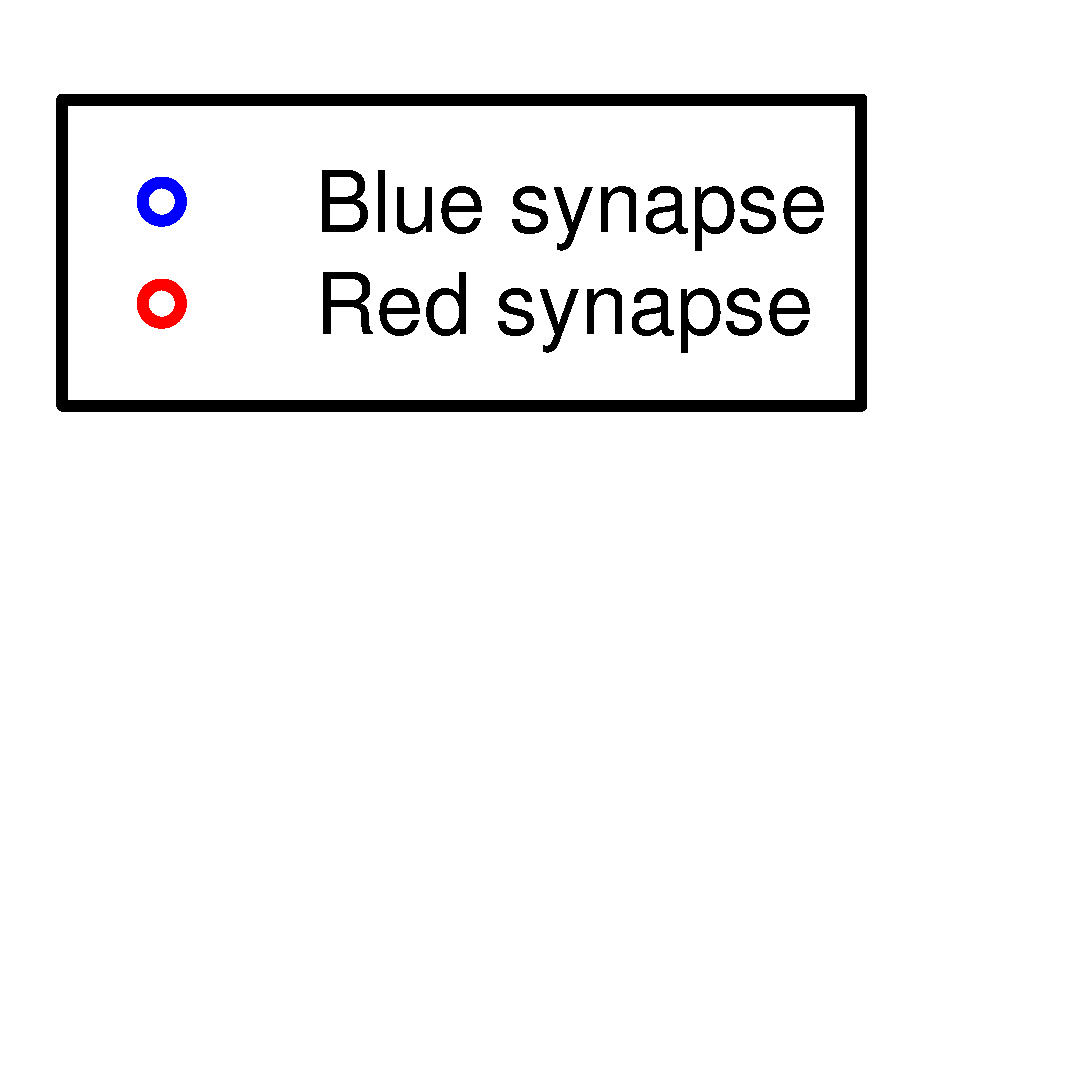
\includegraphics[width=0.35\columnwidth]{./Images_Result/Synapse_legend.eps} 
       \end{subfigure}
       
       \vspace{-3cm}
       \caption{${\Delta}t = 30$[ms], $B$G$N(BKa$B%3%s%@%/%?%s%9J,I[(B}
       \label{k_Ka_dist}
     \end{figure}

     \begin{figure}[H]
       \hspace*{-2cm}
       \begin{subfigure}{0.62\columnwidth}
         \centering
         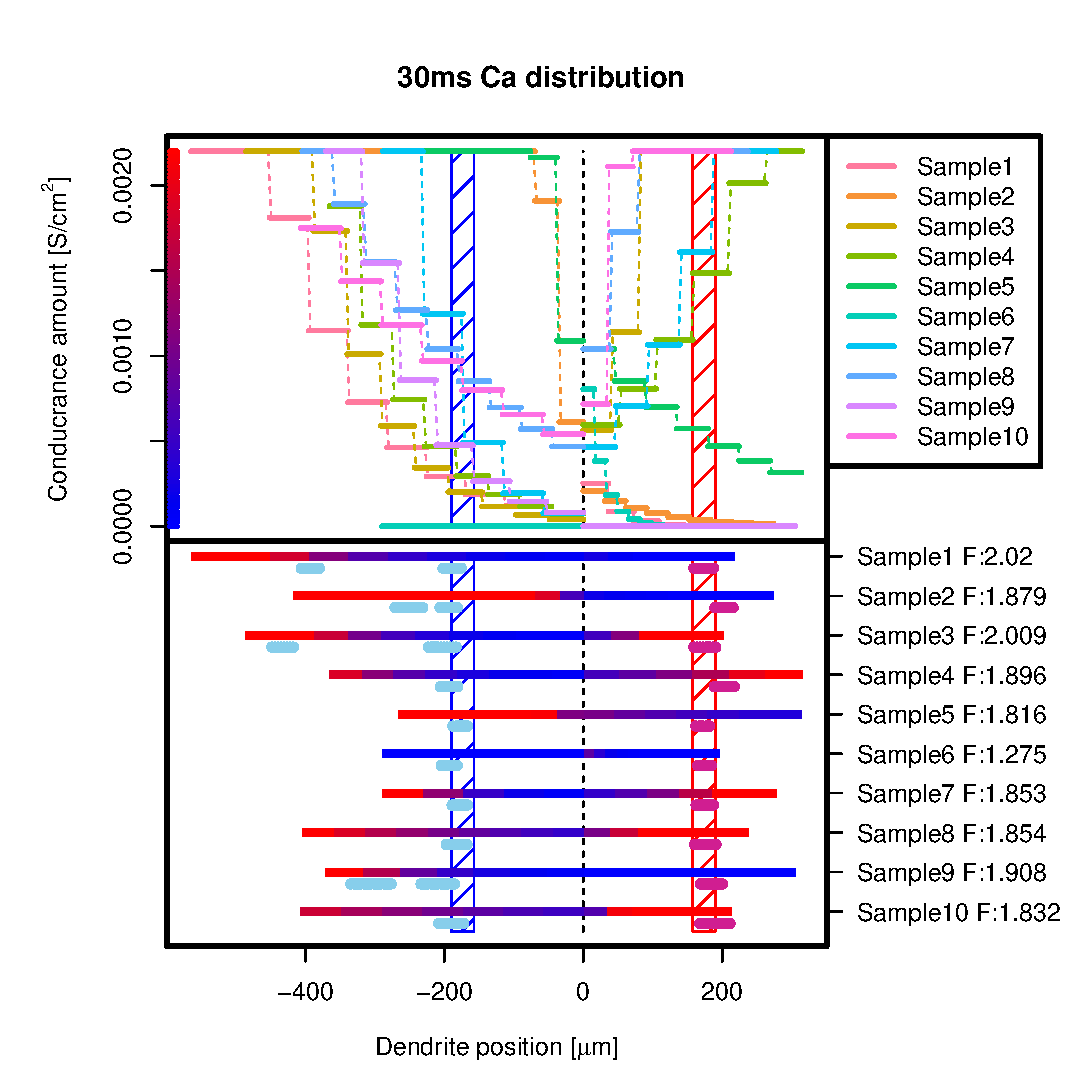
\includegraphics[width=\columnwidth]{./Images_Result/k_ca_Rerative_liner_75_0_Ca_distribution_dt30.eps}
         \caption{$B@~7AJ,I[(B}
         \label{k_liner_reduced_dist}
       \end{subfigure}
       \begin{subfigure}{0.62\columnwidth}
         \centering
         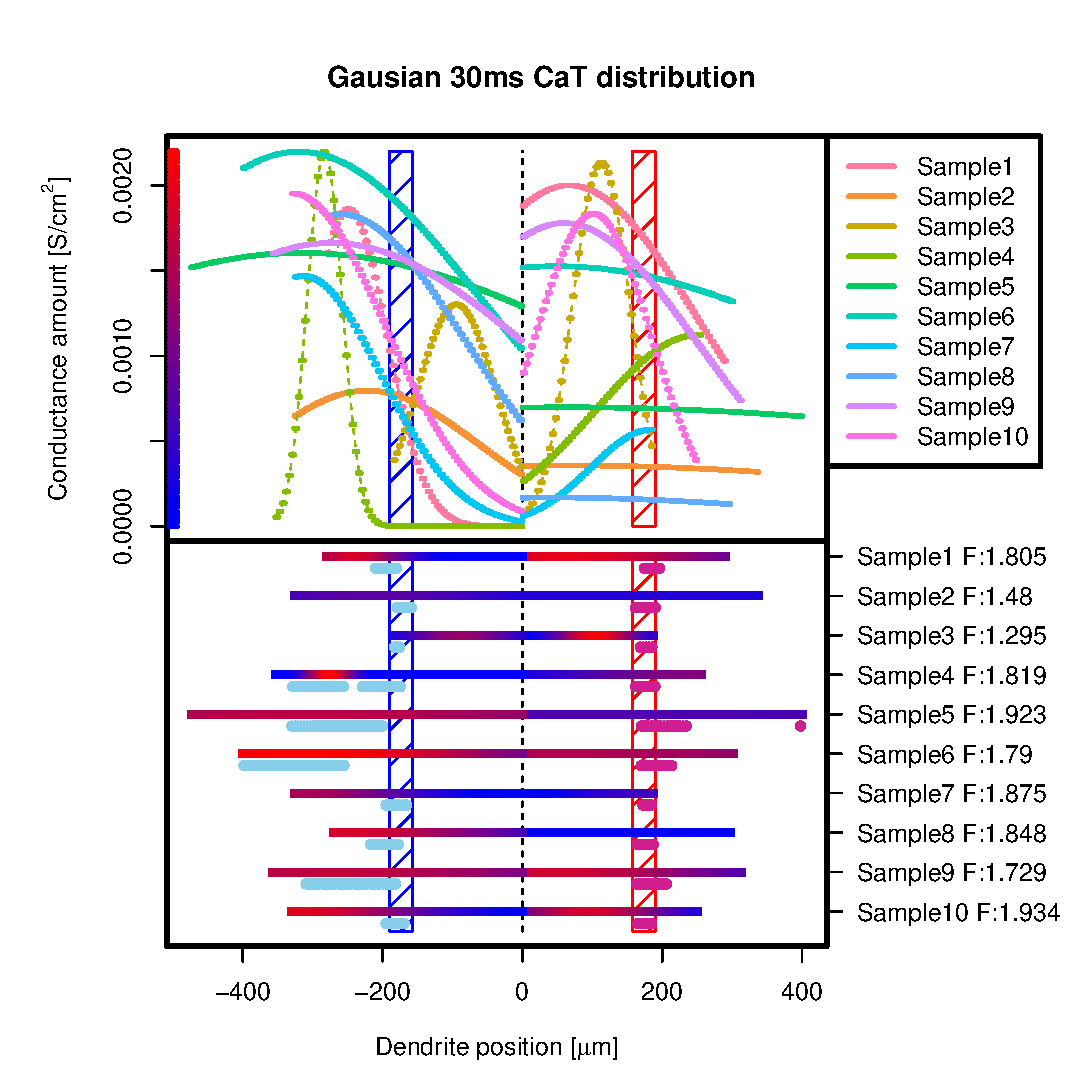
\includegraphics[width=\columnwidth]{./Images_Result/k_ca_Rerative_Gaus_75_0_Ca_distribution_dt30.eps}
         \caption{$B%,%&%9J,I[(B}
         \label{k_gaus_reduced_dist}
       \end{subfigure}

       \hspace*{-2cm}
       \begin{subfigure}{0.62\columnwidth}
         \centering
         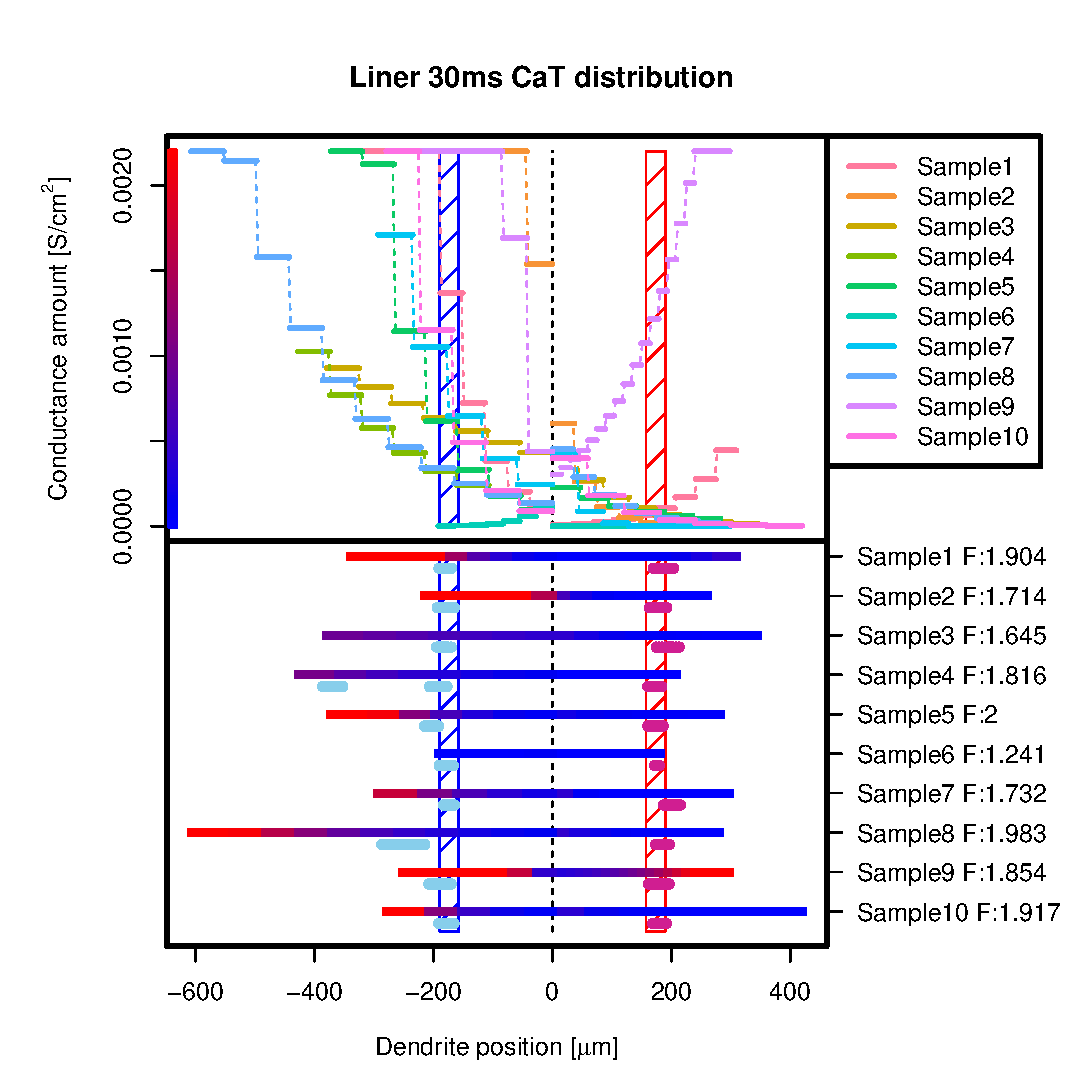
\includegraphics[width=\columnwidth]{./Images_Result/k_ca_Rerative_liner_75_5_Ca_distribution_dt30.eps} %$B$3$l$NBjL>$,(BTsuishi$B$K$J$C$F$k(B
         \caption{$B@~7AJ,I[(B(reduced)}
         \label{k_liner_reduced_dist}
       \end{subfigure}
       \begin{subfigure}{0.62\columnwidth}
         \centering
         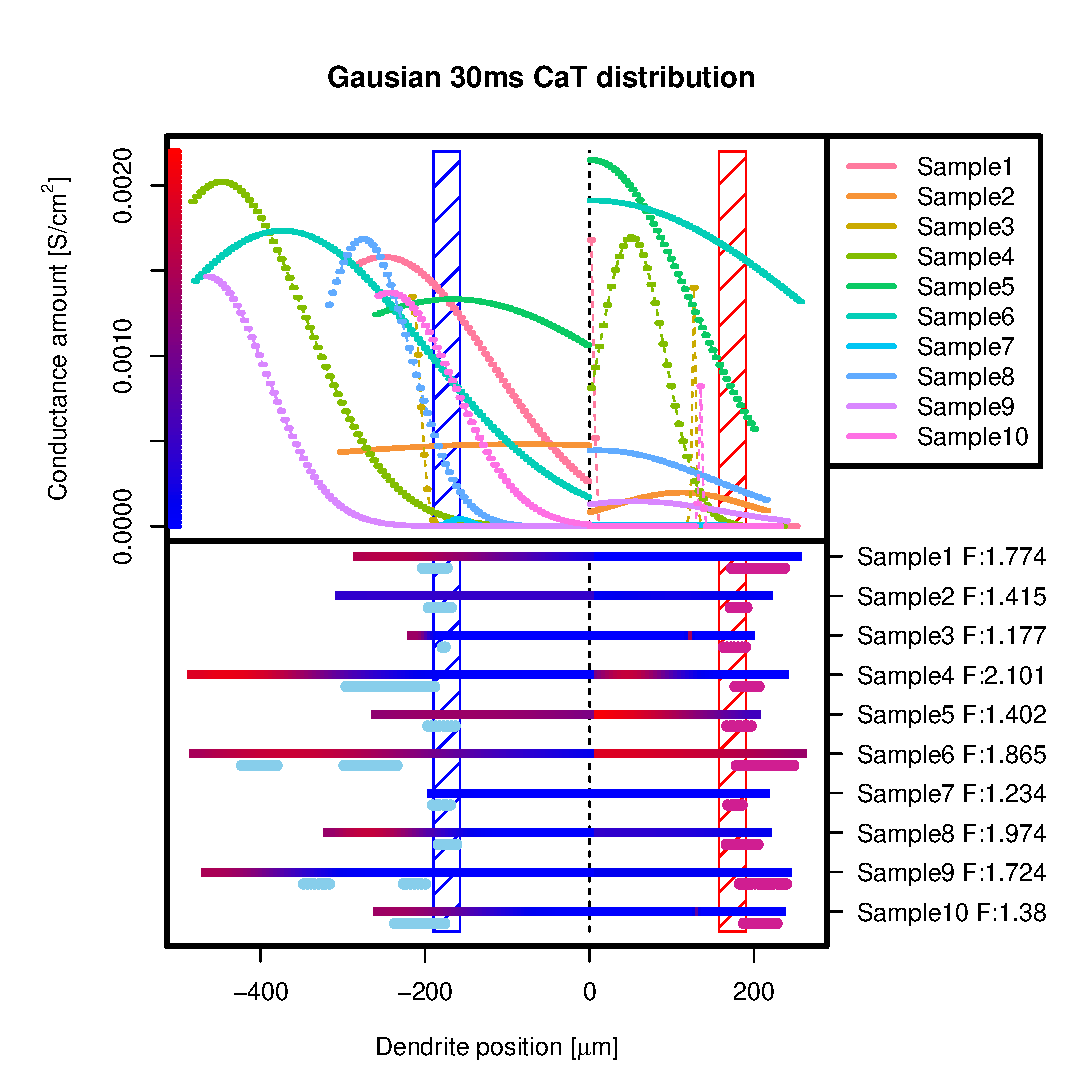
\includegraphics[width=\columnwidth]{./Images_Result/k_ca_Rerative_Gaus_75_5_Ca_distribution_dt30.eps}
         \caption{$B%,%&%9J,I[(B(reduced)}
         \label{k_gaus_reduced_dist}
       \end{subfigure}
       
       \begin{subfigure}{\columnwidth}
         \centering
         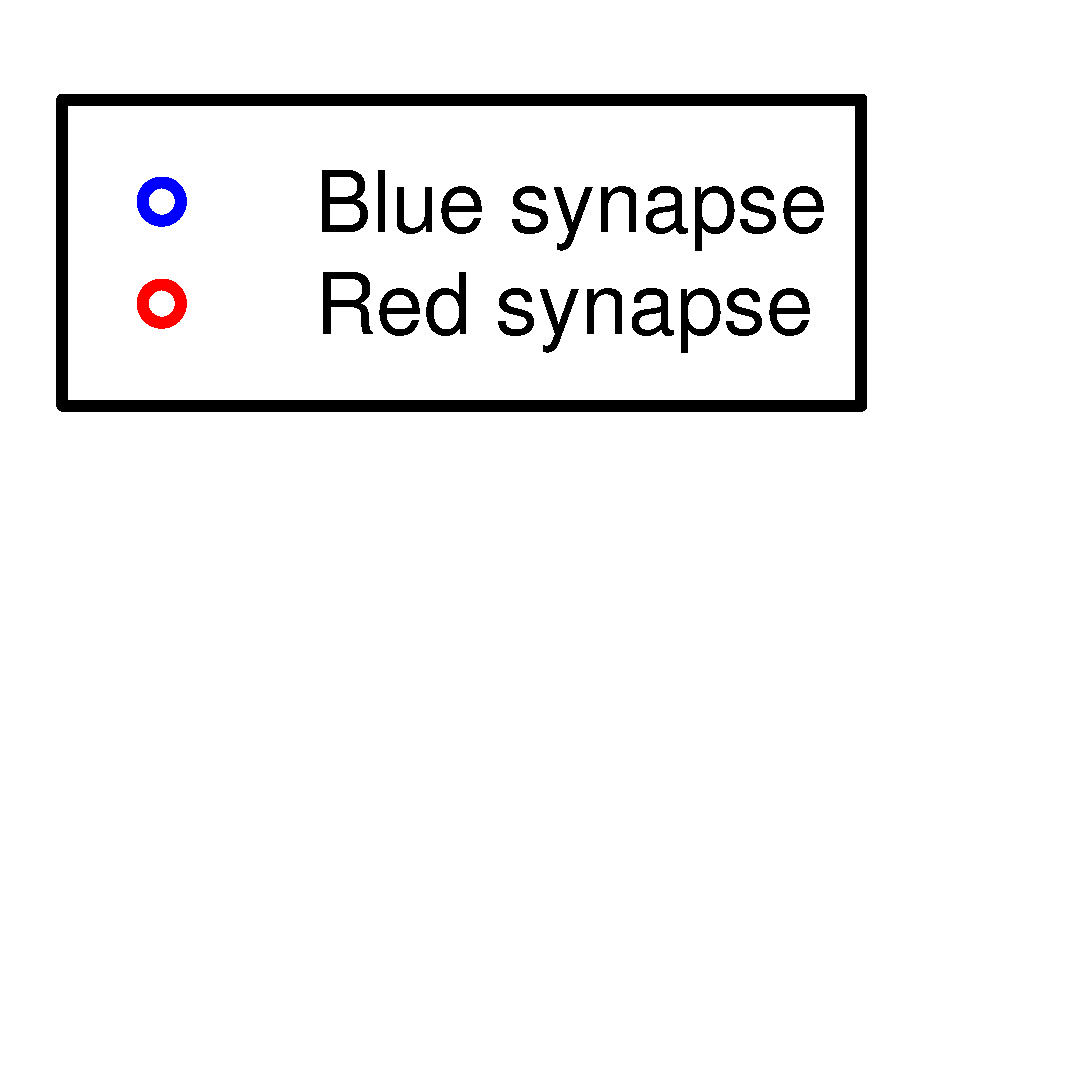
\includegraphics[width=0.35\columnwidth]{./Images_Result/Synapse_legend.eps} 
       \end{subfigure}
       
       \vspace{-3cm}
       \caption{${\Delta}t = 30$[ms], $B$G$N(BCaT$B%3%s%@%/%?%s%9J,I[(B}
       \label{k_CaT_dist}
     \end{figure}
% $B:G8e$K$=$l$>$l$NJ,I[%Q%?!<%s!"%3%s%@%/%?%s%99MN8$NAH$G!"(B4$B%Q%?!<%s$N%3%s%@%/%?%s%9$K$h$k7k2L$r0l$D$N%0%i%U$K$^$H$a$k(B
